%%%%%%%%%%%%%%%%%%%%%%%%%%%%%%%%%%%%%%%%%%%%%%%%%%%%%%%%%%%%%%%%%%%%%%%%%%%%%%%%
%2345678901234567890123456789012345678901234567890123456789012345678901234567890
%        1         2         3         4         5         6         7         8

%\documentclass[letterpaper, 10 pt, conference]{ieeeconf}  % Comment this line out
                                                          % if you need a4paper
\documentclass[a4paper, 10pt, conference]{ieeeconf}      % Use this line for a4
                                                          % paper

\IEEEoverridecommandlockouts                              % This command is only
                                                          % needed if you want to
                                                          % use the \thanks command
\overrideIEEEmargins
% See the \addtolength command later in the file to balance the column lengths
% on the last page of the document



% The following packages can be found on http:\\www.ctan.org
%\usepackage{graphics} % for pdf, bitmapped graphics files
%\usepackage{epsfig} % for postscript graphics files
%\usepackage{mathptmx} % assumes new font selection scheme installed
%\usepackage{times} % assumes new font selection scheme installed
%\usepackage{amsmath} % assumes amsmath package installed
%\usepackage{amssymb}  % assumes amsmath package installed
%\usepackage{hyperref}
\usepackage{bchart}
\usepackage{pgfplots}
\usepackage{subfigure}
\usepackage{float}
\usepackage{amssymb}

%\usepackage[square, numbers, comma, sort&compress]{natbib}

\title{\LARGE \bf
Surgical Activity Recognition in the Operating Room using RGBD Cameras
}

%\author{ \parbox{3 in}{\centering Huibert Kwakernaak*
%         \thanks{*Use the $\backslash$thanks command to put information here}\\
%         Faculty of Electrical Engineering, Mathematics and Computer Science\\
%         University of Twente\\
%         7500 AE Enschede, The Netherlands\\
%         {\tt\small h.kwakernaak@autsubmit.com}}
%         \hspace*{ 0.5 in}
%         \parbox{3 in}{ \centering Pradeep Misra**
%         \thanks{**The footnote marks may be inserted manually}\\
%        Department of Electrical Engineering \\
%         Wright State University\\
%         Dayton, OH 45435, USA\\
%         {\tt\small pmisra@cs.wright.edu}}
%}

% \author{Emre Ozan Alkan$^{1}$, Andru Putra Twinanda$^{2}$, Nicolas Padoy$^{3}$% <-this % stops a space
% \thanks{This work was not supported by any organization}% <-this % stops a space
% \thanks{H. Kwakernaak is with Faculty of Electrical Engineering, Mathematics and Computer Science,
%         University of Twente, 7500 AE Enschede, The Netherlands
%         {\tt\small h.kwakernaak@autsubmit.com}}%
% \thanks{P. Misra is with the Department of Electrical Engineering, Wright State University,
%         Dayton, OH 45435, USA
%         {\tt\small emreozanalkan@gmail.com}}%
% }

% \author{Emre Ozan Alkan$^{1}$, Andru Putra Twinanda$^{2}$ and Nicolas Padoy$^{3}$% <-this % stops a space
% %\thanks{*This work was not supported by any organization}% <-this % stops a space
% \thanks{$^{1}$E. O. Alkan is with Faculty of Electrical Engineering, Mathematics and Computer Science,
%         University of Twente, 7500 AE Enschede, The Netherlands
%         {\tt\small emreozanalkan$@$gmail.com }}%
% \thanks{$^{2}$P. Misra is with the Department of Electrical Engineering, Wright State University,
%         Dayton, OH 45435, USA
%         {\tt\small p.misra at ieee.org}}%
% }

\author{Emre Ozan Alkan$^{1}$, Andru Putra Twinanda$^{2}$ and Nicolas Padoy$^{2}$% <-this % stops a space
%\thanks{*This work was not supported by any organization}% <-this % stops a space
\thanks{$^{1}$E. O. Alkan is with,
        University of Bourgogne, France.
        {\tt\small emreozanalkan$@$gmail.com}}%
\thanks{$^{2}$A. P. Twinanda and N. Padoy are affiliated to ICube Laboratory, University of Strasbourg, France.
        {\tt\small \{twinanda, npadoy\}$@$unistra.fr}}%
}



\begin{document}



\maketitle
\thispagestyle{empty}
\pagestyle{empty}


%%%%%%%%%%%%%%%%%%%%%%%%%%%%%%%%%%%%%%%%%%%%%%%%%%%%%%%%%%%%%%%%%%%%%%%%%%%%%%%%
\begin{abstract}

Operating room management and surgical procedure evaluation are time consuming tasks for operating room managers and clinicians. The demanding workload can be reduced thanks to context-aware systems that use signals and data from operating rooms to automate processes such as surgical skill analysis, transcription of medical produces and evaluation of quality of procedures. Activity recognition is one of the key factors to enable the context-aware systems in the operating rooms. In this work, we address the problem of activity recognition in an operating room using a multi-view RGBD camera system. We adopt the activity recognition pipeline based on bag-of-words (BoW) approach by \cite{c1} and extend it with a 4D spatio-temporal voting scheme.  In the recognition pipeline, a data-driven non-rigid layout is learnt to divide the 4D spatio-temporal space of the features into 4D patches in order to recover the information loss caused by the BoW approach. Since each patch from the learnt layout carries meaningful and semantic information of the 4D spatio-temporal space for an activity, the proposed voting scheme collects votes from the patches to determine the activity. We tested the proposed method on a multi-view RGBD dataset using two classifiers, i.e., Support Vector Machines (SVM) and Random Forest (RF). We also compare the results of the proposed voting scheme approach to the non-voting approach \cite{c1}. The experiments show that the proposed voting scheme shows promising results with 83.1\% accuracy.

\end{abstract}


%%%%%%%%%%%%%%%%%%%%%%%%%%%%%%%%%%%%%%%%%%%%%%%%%%%%%%%%%%%%%%%%%%%%%%%%%%%%%%%%
\section{INTRODUCTION}
\label{sec:introduction}

% Activity recognition using cameras is a very active research topic since the past several decades in the domain of computer vision. It has been widely applied in many fields, such as video surveillance, human computer interaction, robotics and medicine. However, activity recognition is still a very challenging problem due to the large amount of data, amount of computational power required, and high intra-class variations of activities. Over the past decades, researchers have mainly focused on using image sequences from single-view RGB cameras for activity recognition which have many inherent limitations. Single-view camera approaches have limitations due to narrow field of view which makes it more vulnerable to occlusions. Moreover, RGB cameras are very sensitive to illumination changes. 

Recent technological advances and the emergence of cost-effective depth sensors, depth cameras have become more popular and attracted many researchers to use them in activity recognition studies. Depth sensors have many advantages over RGB cameras. For example, they can provide structural information of the scenes and they can even work in total darkness since infrared structured light is used to reconstruct the scenes. All these advantages make it interesting to incorporate the RGBD cameras into a more challenging environments, e.g., operating rooms (OR).

Recent progresses in medicine transformed ORs into hybrid rooms equipped with new imaging devices, robotic arms, sensors and electronic devices. These changes require more management and tracking of information. Therefore, activity recognition in ORs has become an important research field in the domain of medicine. It enables applications, such as OR time management for hospitals \cite{c2}, surgical work-flow modeling and monitoring \cite{c4}, surgical skill analysis \cite{c5} and automatic transcription of medical procedures \cite{c6}. In particular, activity recognition in ORs equipped with x-ray imaging devices can be used to estimate  the radiation exposure of the patients and the clinicians and correlate it to their activities \cite{c7}. 

% In order to recognize activities, many data sources from operating rooms can be used, e.g, the vital signs of the patients \cite{Bhatia:2007:RIO:1620113.1620126} and tool usage signals \cite{Padoy2012632}. However, they are only providing local information that is not enough to capture global activities and events in the operating room. Thus, in this thesis, we focus on performing activity recognition on videos. Specifically we are identifying what activities is happening in a video clip.

% \cite{twinanda2015data} have addressed the same problem. In their work, they proposed an action recognition pipeline with a novel feature encoding scheme that achieved 85.53\% accuracy. The proposed novel feature encoding extends the bag-of-words (BoW) approach to learn a data-driven non-rigid layout to divide the 4D spatio-temporal (3D spatial + 1D temporal) space of the feature locations. Their work showed that encoding features with the learned non-rigid layout retains more spatio-temporal information compared to the rigid counterpart, i.e, SPM \cite{1641019}. 

In this paper, we propose to adopt the activity recognition pipeline from \cite{c1} and extend it with a voting scheme to solve activity recognition in the OR using video clips. Firstly, interest points are detected from intensity and depth video clips. Secondly, features are extracted around the detected interest points. Then we learn two separate dictionaries to encode our extracted features. A visual dictionary is learned to encode visual features. On the other hand, the spatio-temporal dictionary is learned to define a 4D non-rigid layout. The non-rigid layout divides the 4D spatio-temporal space into smaller 4D patches. We also introduce two voting approaches: one-model and multi-model. In the one-model approach, each patch from all video clips are used to train a classifier. On the other hand, the multi-model approach trains a separate classifier for each patch. In order to provide a comprehensive comparison, we present the results for voting sheme and non-voting scheme approaches using non-linear SVM and RF classifiers.

% In this paper, we propose to adopt the activity recognition pipeline from \cite{c1} and extend it with a voting scheme to solve activity recognition in the OR using video clips. Firstly, spatio-temporal interest points (STIP) and depth spatio-temporal interest points (DSTIP) are detected from intensity and depth video clips respectively. Secondly, histogram of optical flows (HOF) from intensity and depth cuboid similarity features (DCSF \cite{c9}) from depth data are extracted around the detected interest points. Then we learn two separate dictionaries to encode our extracted features. A visual dictionary is learned to encode visual features: the HOF and the DCSF. On the other hand, the spatio-temporal dictionary is learned to define a 4D non-rigid layout. The non-rigid layout divides the 4D spatio-temporal space into smaller 4D patches. From each patch, a histogram of feature points will be counted. Finally, histograms coming from the same video clip will be passed to the classifiers to vote for the action. We also introduce two voting approaches: one-model and multi-model. In the one-model approach, each patch from all video clips are used to train a classifier. On the other hand, the multi-model approach trains a separate classifier for each patch. In order to provide a comprehensive comparison, we present the results for voting sheme and non-voting scheme approaches using non-linear SVM and Random Forest classifiers.

% The rest of the paper is organized as follows. Section~\ref{section:relatedWork} introduces the related work on activity recognition. Section~\ref{section:methodology} provides the details of the methodology used in this work. Section~\ref{section:experiments} describes and discusses the experimental setup and results. Finally, Section~\ref{section:conclusionsAndFutureWorks} presents the conclusions of the paper.

%%%%%%%%%%%%%%%%%%%%%%%%%%%%%%%%%%%%%%%%%%%%%%%%%%%%%%%%%%%%%%%%%%%%%%%%%%%%%%%%
\section{RELATED WORK}
\label{section:relatedWork}

	The problem of activity recognition has been widely studied in the computer vision field. Recent works show excellent performances using local features such as local motions \cite{c10, c11}, human detectors \cite{c12} and skeleton tracking \cite{c13}. In \cite{c11}, Yang et al. presented an activity recognition framework for depth sequences. Clustered hypersurface normals are used to construct polynormals to get shape information from depth sequences. The method achieved good results on public Microsoft human action dataset MSR \cite{c17}. However, super normal vectors (SNV) encoded method is not reliable either on a highly cluttered and occluded environment or when the actions have very low depth variance.

% 	More recently, great improvements were obtained by using skeleton tracking based activity recognition approaches. \cite{6909476} proposed a novel skeleton representation that is modeling the 3D geometric relationships between various body parts. They outperformed most of the skeleton-based state-of-the-art methods with their representation. In other work, \cite{6909731} argues that skeleon-based approaches are limited by the effective working distance of the RGBD cameras and practically they are not online all the time. They proposed using the combination of intensity, depth and skeleton structures. In \cite{6909735}, Want et al. stated that action recognition is view-dependent and proposed a novel multiview spatio-temporal graphical representation for cross-view action recognition. The proposed method leverages from 3D human skeleton data. Despite the satisfactory performance of skeleton tracking approaches, frontal camera views of the persons with low occlusion is needed which are not always possible in environments such as the operating rooms. \cite{RahimKinectOR} addressed the problem of skeleton tracking of clinicians in the operating rooms and showed that off-the-shelf skeleton tracking methods fail most of the time.
    
 	In one of the most related work with a multi-view systems and voting scheme, Zhu et al. \cite{c22} addressed the problem of multi-view activity recognition using voting scheme and random forest classifier. They use IXMAS human action dataset \cite{c24} which consist of 5 cameras, 13 daily-live actions with various data, e.g., silhouettes, reconstructed volumes. However, the dataset does not consist of real activities, i.e., the dataset is recorded in a laboratory environment. The method is dependent on the extracted 2D silhouettes from each camera. The segments in temporal domain consist of 2D binary silhouettes which are used to train the RF classifier to get prediction histograms used in voting. The voting strategy collects the vote from each segment of video clip and apply the weights on the features and on the camera views. Their results showed that combination of multi-view cameras, voting scheme and RF classifier produce good results. On the other hand, in multi-view camera systems, actions may not be available from each camera view all the time. Furthermore, methods, like silhouette extraction or human tracking are not feasible to be used in highly cluttered environments, e.g., ORs.
    
    The problem of activity recognition in the OR using a multi-view camera system is not a trivial problem because of various challenges. Firstly, camera positioning in ORs for better field of view while accommodating the articulation of the surgical equipments is very challenging. In addition, ORs are very dense and dynamic with a cluttered background and reflective objects, high occlusions, illumination changes, upfront camera view and very tiny or slow movements. Hence, methods in \cite{c11, c13, c20} are not sufficient to deal with these problems. Due to these difficulties, it is required to have lower level features to represent the video clips.
    
%     One example of the lower level features for an image sequence is spatio-temporal interest point (STIP)\cite{ laptev2005space}. STIPs are sparse interest points along spatial and temporal domain, which are detected by Harris corner detection in 3D spatio-temporal domain. In \cite{1570899}, Dollar et al. proposed a modified sparse and informative STIP and showed that it is robust to pose, clutters and occlusions. The STIPs \cite{1570899} are described with cuboids extracted from surrounding spatio-temporally windowed data. The proposed interest points are more robust to gradual gradient changes and periodic movements. However, the approach was designed to work mainly for intensity data and did work properly on depth data because of the nouse. \cite{6619209} proposed filtering method to detect STIP in depth data, namely depth spatio-temporal interest points (DSTIP). They also introduced a novel feature (i.e., Depth Cuboid Similarity Feature) to describe local similarity of 3D depth cuboids around DSTIP.
    
    In a recent work \cite{c1}, Twinanda et al. showed that intensity or depth data is not sufficient by itself to recognizing some actions in the ORs. Some actions are well recognized in depth videos due to illumination problems in intensity data, and some actions give better results in intensity data due to low depth variance of depth data. Hence, the combination of both intensity and depth data have more discriminating power than using only intensity or depth data. The problem of activity recognition in an OR using multi-view RGBD camera systems was addressed. A dataset of 1734 video clips of 15 surgical activity is generated using 2 RGBD cameras from real surgical operations in a hybrid OR. Achieving 85.53\% accuracy, the work showed that encoding features with a non-rigid layout retains more spatio-temporal information compared to Spatial Pyramid Matching (SPM) \cite{c8}.
    
%Then, STIP \cite{c26} and DSTIP \cite{c9} are detected from intensity and depth respectively. They extracted HOF and DCSF \cite{c9} features around the STIP and DSTIP respectively. These features are encoded by a novel feature encoding scheme that extends the BoW approach to learn a non-rigid layout that divides the 4D spatio-temporal space of the feature locations. Achieving 85.53\% accuracy, the work showed that encoding features with the non-rigid layout retains more spatio-temporal information compared to Spatial Pyramid Matching (SPM) \cite{c8}.


\addtolength{\textheight}{-3cm}   % This command serves to balance the column lengths
                                  % on the last page of the document manually. It shortens
                                  % the textheight of the last page by a suitable amount.
                                  % This command does not take effect until the next page
                                  % so it should come on the page before the last. Make
                                  % sure that you do not shorten the textheight too much.

%%%%%%%%%%%%%%%%%%%%%%%%%%%%%%%%%%%%%%%%%%%%%%%%%%%%%%%%%%%%%%%%%%%%%%%%%%%%%%%%
\section{METHODOLOGY}
\label{section:methodology}

% 	In this section, the adopted activity recognition pipeline from \cite{twinanda2015data} and the proposed voting scheme are explained in detail with various classification strategies.

%----------------------------------------------------------------------------------------

\subsection{Adopted Classification Pipeline \cite{c1}}
\label{section:AdoptedClassificationPipeline}
The adopted pipeline \cite{c1} is as follows: acquisition from a multi-view camera setup, interest point detection, feature extraction and building a data-driven non-rigid layout for feature encoding.

%----------------------------------------------------------------------------------------
\subsubsection{Multi-View RGBD Camera Setup}
\label{section:MultiViewRGBDCameraSetup}
    The proposed multi-view camera system contains two RGBD sensors, i.e. Asus XtionPro Live, mounted on the ceiling of the OR. The cameras record both intensity and depth data synchronously at 14 fps with 640 x 480 resolution. 
%     While one of the sensors is capturing the area around the operating room bed, the other sensor captures the area with equipment table, in which large area of the operating rooms is covered.
%     Furthermore, thanks to minimal overlapping of the views of the sensors, interference of infrared patterns of depth sensors are very less. 
    The intrinsic parameters for each camera are obtained by calibration with checkerboard pattern. The extrinsic parameters are obtained  by using laser pointer method described in \cite{c27}. Both camera views are shown in Figure~\ref{fig:cameraViews}.
    
\begin{figure}
\centering
\subfigure[Camera view 1 - intensity data]{\label{sfig:view1Intensity}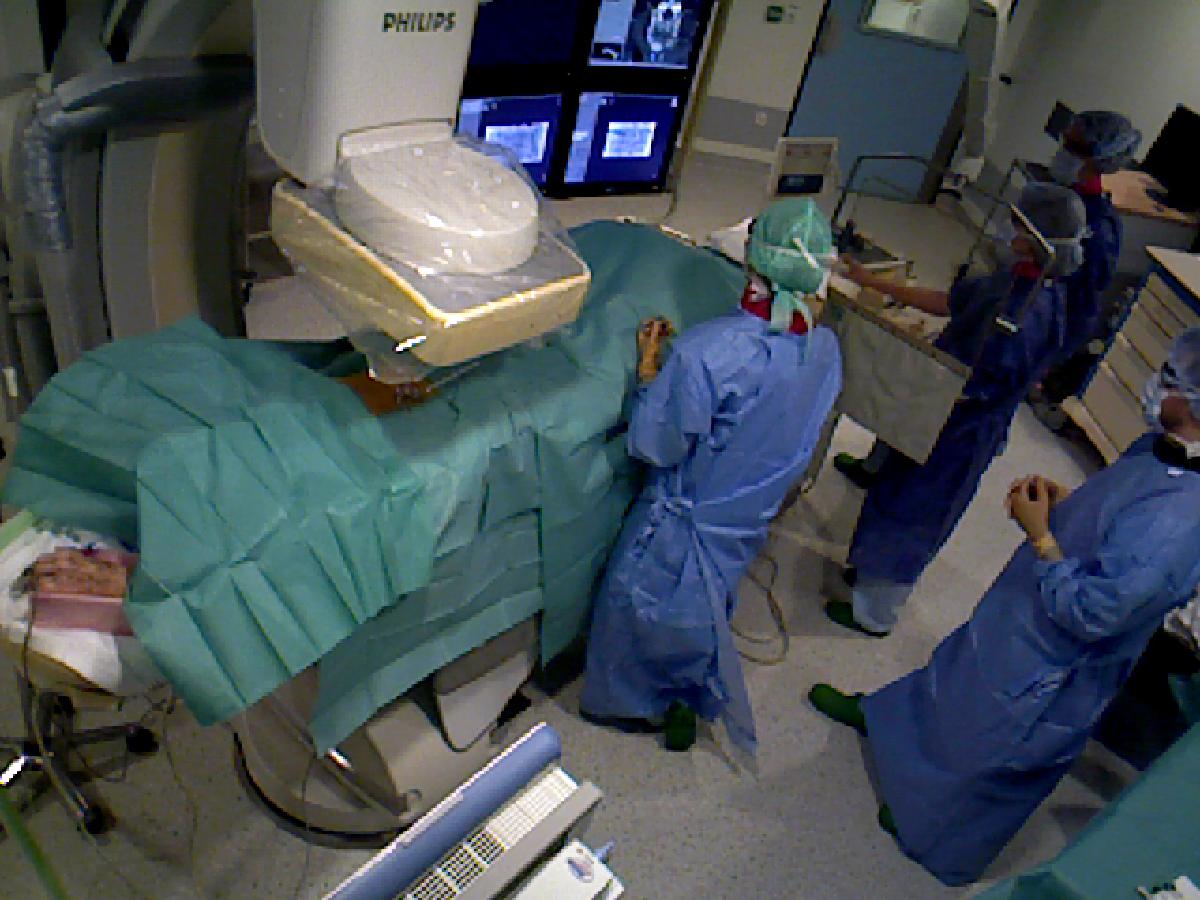
\includegraphics[width=.20\textwidth]{Figures/View1Color}}
\subfigure[Camera view 1 - depth data] {\label{sfig:view1Depth}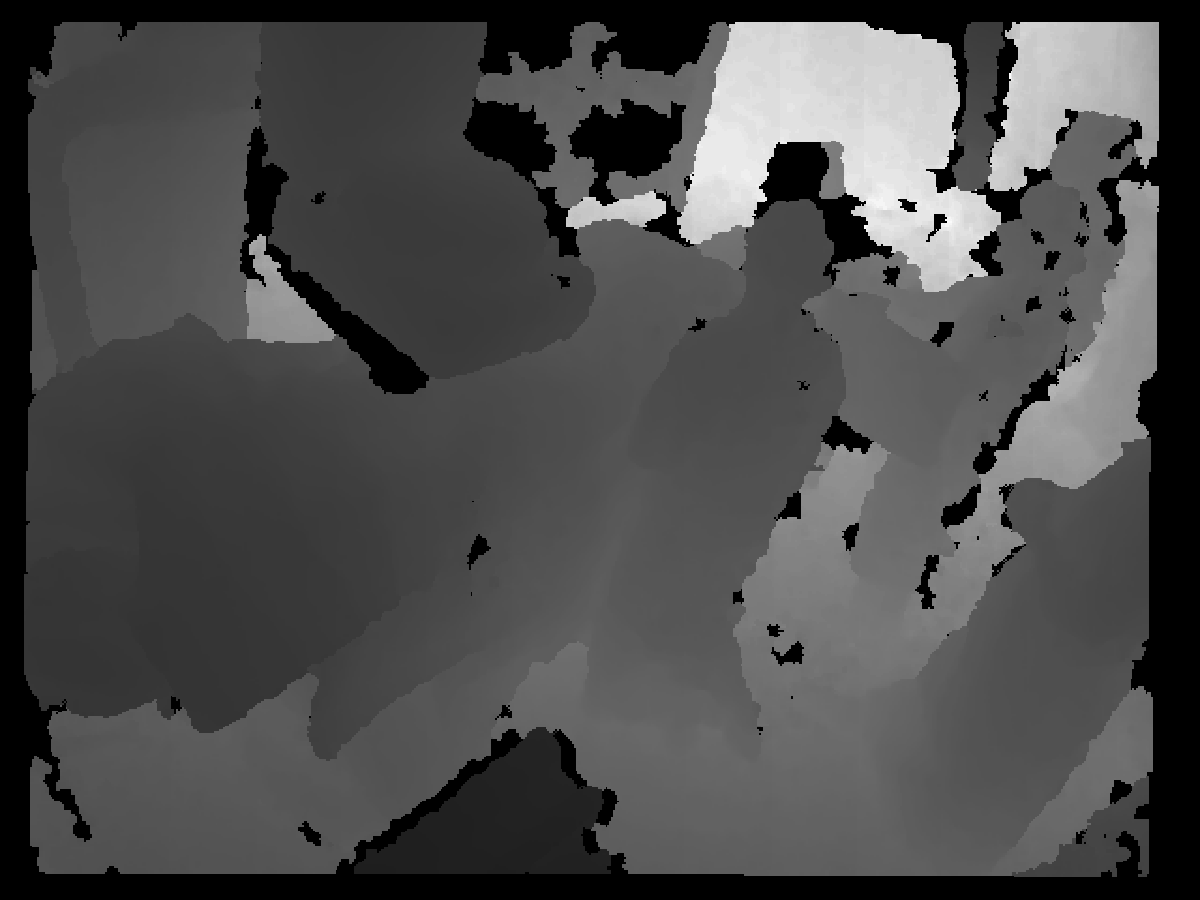
\includegraphics[width=.20\textwidth]{Figures/View1Depth}}\\
\subfigure[Camera view 2 - intensity data]{\label{sfig:view1Intesity}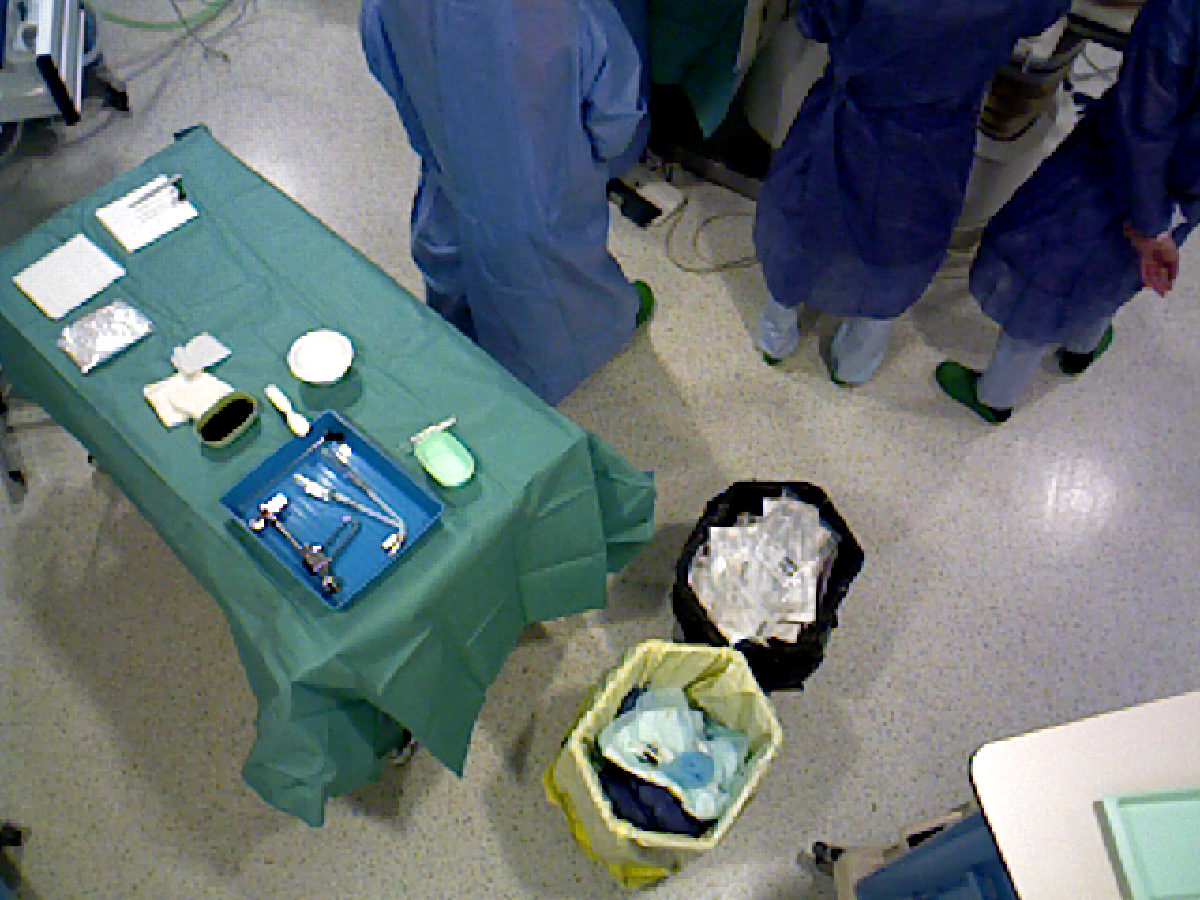
\includegraphics[width=.20\textwidth]{Figures/View2Color}}
\subfigure[Camera view 2 - depth data]{\label{sfig:view2Depth}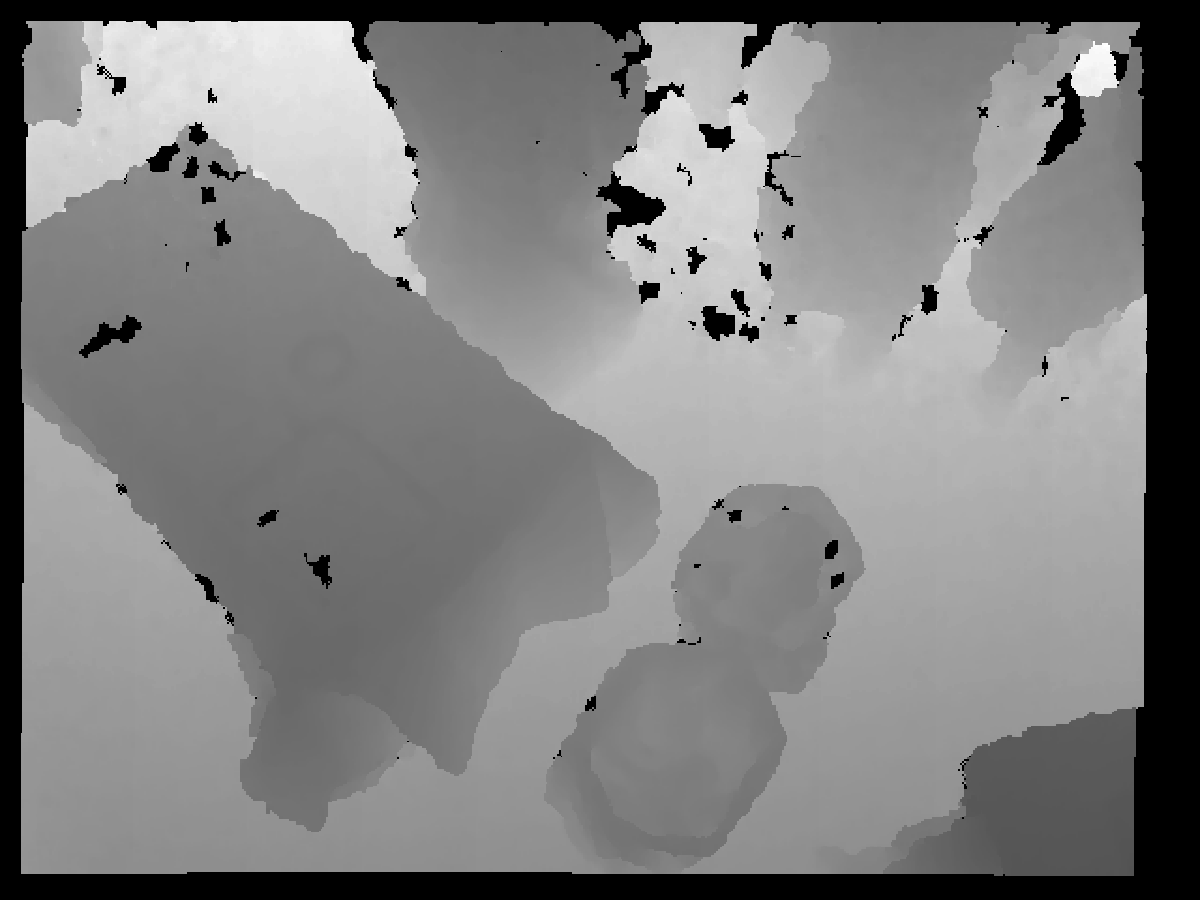
\includegraphics[width=.20\textwidth]{Figures/View2Depth}}\\
\caption{Sample images from RGBD sensors with view 1 and view 2.}
\label{fig:cameraViews}
\end{figure}
%----------------------------------------------------------------------------------------
\subsubsection{Interest Point Detection}
\label{section:InterestPointDetection}
	In the activity recognition pipeline, STIP \cite{c26} are used for intensity data. STIPs are computed by applying separable linear filters to get local maximum of the response. The response fuction $R$ of an intensity image $I$ is calculated as follows:

\begin{equation}
R_{I} = \left(I * g * h_{even}\right)^{2} + \left(I * g * h_{odd}\right)^{2},
\label{eq:stipResponseFunction}
%\nonumber
\end{equation}

	where $g(x, y; \sigma)$ is the 2D Gaussian smoothing kernel with scale $\sigma$, applied on the spatial $\left(x, y\right)$ dimensions. Terms $h_{even}$ and $h_{odd}$ are the quadrature pair of 1D Gabor filters applied in temporal domain defined as: $h_{even}\left(t|\tau,\omega,\right)=\cos\left(2\pi\omega t\right)e^{\frac{-t^{2}}{2\tau^{2}}}$ and $h_{odd}\left(t|\tau,\omega\right)=\sin\left(2\pi\omega t\right)e^{\frac{-t^{2}}{2\tau^{2}}}$.
    
    However, the STIP detector does not perform well and falsely detected on depth data because of the nature of the depth data where it may contain noise from sensors and pattern interference. In order to cope with these problems, DSTIP detector by \cite{c9} is used to detect depth spatio-temporal interest points (DSTIP) on depth data which introduced filtering method to reduce the noise and the false detection. Additional noise suppression term is proposed for noise filtering to equation \ref{eq:stipResponseFunction}:

\begin{equation}
R_{D} = \left(D * g * h_{even}\circ\bar{s}\right)^{2}+\left(D * g * h_{odd}\circ\bar{s}\right)^{2},
\label{eq:dstipResponseFunction}
%\nonumber
\end{equation}

where $D$ is the depth image, and $\bar{s}$ is the noise suppression term.


%----------------------------------------------------------------------------------------
\subsubsection{Feature Extraction}
\label{section:FeatureExtraction}
We compute features by extracting 3D cuboid around each detected interest points in spatio-temporal location $\left(x, y, t\right)$. The size of the cuboids $\left(\Box_{x}\times\Box_{y}\times\Box_{t}\right)$ is proportionally assigned according to the spatial scale $\sigma$ and the temporal scale $\tau$.

Intensity cuboids are extracted from intensity data and HOF are calculated from the intensity cuboids. HOFs are used in intensity feature extraction process due to its distinguishable properties for direction of motion. These properties help to distinguish activities which have similar movements with different directions.

Moreover, 3D depth cuboids are extracted from depth data. Then, the DCSF \cite{c9} are computed from the cuboids. DCSFs are computed based on self-similarity to encode spatio-temporal structure of the 3D cuboid. %DCSF divides cuboids into smaller voxels, compute histograms of the depth pixels from each voxel, calculating relationship of each voxel by defining similarity between voxels using Bhattacharyya distance, then combination of all similarity scores from the voxels are concatenated to generate a DCSF feature.

%----------------------------------------------------------------------------------------
\subsubsection{Data Driven Feature Encoding}
\label{section:DataDrivenFeatureEncoding}

% 	The BoW is a model that treats image features as words to construct vocabulary. Then, histogram of occurrences of the words from the vocabulary produces a sparse histogram vector. $K$-means is typically used to encode the features which provide a global representation with BoW where $\mathbf{x}$ is a feature, $ \forall \mathbf{x} $, a value $w\in\left\{ 1,\cdots,K\right\}$, where $K$ is number of $K$-means center, is assigned to describe the index of the $K$-mean center which is the closest to feature $\mathbf{x}$. Hence $K$-means clusters every feature vector $\mathbf{x}\in\mathbb{R}^{n}$ and express them in a sparse representation $\mathbf{s}\in\mathbb{R}^{K}$ which is the occurrences of the words from the learnt dictionary $\mathbf{D}\in\mathbb{R}^{n\times K}$

	In \cite{c1}, learning two separate dictionaries are proposed: a visual dictionary $\mathbf{D_{v}}$ with $K_{v}$ centers and a spatio-temporal dictionary $\mathbf{D_{st}}$ with $K_{st}$ centers. The visual dictionary $\mathbf{D_{v}}$ is learnt for encoding the visual features, i.e., the HOF and the DCSF for representing video clips. On the other hand, the spatio-temporal dictionary $\mathbf{D_{st}}$ is learnt by clustering the locations of the interest points $\left(x,y,z,t\right)$, where $X=\left(x,y,z\right)$
and $t$ are the 3D coordinates and the temporal location
of the interest point, respectively. Since the video clips varies in length, $t$ is normalized by length of its video clip. 

% Multi-view camera systems require to define one camera's coordinate system as a reference coordinate system to transform the 3D coordinates into a common coordinate system. Hence, the final 3D coordinates are computed by:

% \begin{equation}
% \begin{array}{c}
% X=T_{R}\cdot Y+T_{t}\\
% Y=d\cdot C^{-1}\cdot\left(\begin{array}{ccc}
% u & v & 1\end{array}\right)^{\top},
% \end{array}
% \end{equation}

% where $Y$ is the 3D point in the camera frame, $\left(u,v\right)$
% and $d$ are respectively the image pixel coordinates and the corresponding
% depth value, $C$ is the intrinsic camera matrix, $T_{R}$
% and $T_{t}$ are respectively the rotation and translation from the
% camera frame to the reference frame. 

Then, learnt spatio-temporal dictionary $\mathbf{D_{st}}$ is used to place a non-rigid spatio-temporal grid to divide the spatio-temporal space into patches $\{P^{1},...,P^{K_{st}}\}$. These local patches from the non-rigid layout are high dimensional 4D patches. 

%One example of feature encoding in 2D space is shown in Figure~\ref{fig:featureEncoding} where non-rigid layout is learnt by clustering points indicated with colored patches and features are extracted from the patches.

% \begin{figure}[htbp]
% \begin{center}
% 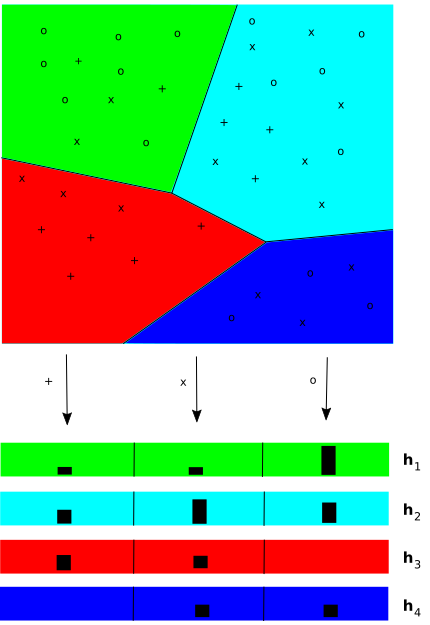
\includegraphics[scale=0.4]{Figures/featureEncoding2}
% \end{center}
% \caption{Example of data driven feature encoding in 2D space with $K_{v}$ = 3 and $K_{st}$ = 4\label{fig:featureEncoding}}
% \end{figure}
    
	In order to get the final histogram representation of the patches for a video clip $V_{i}$, where $i$ is video instance count, firstly, all features, $\forall \mathbf{x}$, belong to their corresponding patch, $P^{j}$, are found using the $\mathbf{D_{st}}$. Secondly, using the $\forall \mathbf{x} \in P^{j}$, the histogram of visual word occurrences from every patch $P^{j}$ is computed using $\mathbf{D_{v}}$. Finally, we obtain $K_{st}$ histograms, $\{_{i}H^{1},..., _{i}H^{K_{st}}\}$, representing the patches $P^{j}$ from video clip $V_{i}$, where $_{i}H^{j} \in \mathbb{R}^{K_{v}}$.
%----------------------------------------------------------------------------------------
\subsection{Voting Scheme}
\label{section:VotingScheme}
We extended the pipeline aforementioned by proposing a voting scheme. The proposed voting scheme uses histograms $H^{j}$ obtained from patches $P^{j}$ of a data-driven non-rigid layout presented in Section~\ref{section:DataDrivenFeatureEncoding}. We classify every local patch $P^{j}$ using $H^{j}$ independently and collect their vote for calculating majority vote for global activity. Hence every patch $P^{j}$ holds information about activity with semantic information that is contributing globally. 

%----------------------------------------------------------------------------------------
\subsection{Activity Classification}
\label{section:ActionClassification}

	In our multi-view camera system, every activity $a_{i}$ is recorded from both of the views. Hence, it produces a video clip pair $\left(V_{i}^{1},V_{i}^{2}\right)$ from the cameras. Firstly, interest point detection in Section~\ref{section:InterestPointDetection} is applied on the video clip pair $\left(V_{i}^{1},V_{i}^{2}\right)$ and features are extracted as described in Section~\ref{section:FeatureExtraction}. Then, two dictionaries are learnt for encoding as described in Section~\ref{section:DataDrivenFeatureEncoding}. The learnt spatio-temporal dictionary divides 4D space into smaller local 4D patches $\{P^{1},...,P^{K_{st}}\}$. Then, histogram representation $H^{j}$ from each local patch $P^{j}$ is calculated using the learnt visual dictionary for the video clip pair $\left(V_{i}^{1}, V_{i}^{2}\right)$. In order to get final histogram representation, $\{_{i}H^{1},..., _{i}H^{K_{st}}\}$, for video clip pair $\left(V_{i}^{1},V_{i}^{2}\right)$, we merge information by computing $_{i}H^{j} = _{i}^{1}H^{j} + _{i}^{2}H^{j}$ where $_{i}^{1}H^{j}$ and $_{i}^{2}H^{j}$ are respectively histograms from patch $P^{j}$ of $V_{i}^{1}$ and $V_{i}^{2}$. Then, final histograms, $\{H^{1},..., H^{K_{st}}\}$ from all video clip pairs are passed to the classifier for training and testing. 
    
%In order to make performance comparison, we use the one-against all Support Vector Machine (SVM) with the nonlinear kernel, and we use Random Forest implementation to give comprehensive comparison of the voting scheme.


% \subsubsection{Training Strategy}
% \label{section:TrainingStrategy}
In this work, we propose to use a two-level classification strategy to carry on the voting scheme. In the first level, we learn a classification model to obtain the probability votes from the 4D patches. However, in the second level classification, we learn the weights for the probability votes under the assumption that each patch has different contribution. In addition to the proposed training strategy, we also propose to use two different approaches used in the first level of the proposed classification strategy, i.e., one-model and multi-model approaches. In the one-model approach, all histograms from each patch from each video is trained using one classifier. However, in the multi-model approach, separate classifiers are trained for each patch.

\subsubsection{One-Model Approach}
\label{section:OneModelApproach}
In one-model approach, we use one classifier model in each level, i.e., $M_{level1}$ and $M_{level2}$. First, we train $M_{level1}$ with the training set which consists of a collection of histogram vectors $\{H^{1}, ..., H^{K_{st}}\}$. Then, we pass the histogram vectors to $M_{level1}$ to get the probability votes $\{W^{1}, ..., W^{K_{st}}\}$ from each video clip pair where $W^{j} \in \mathbb{R}^{N_{c}}$ and $N_{c}$ is the number of activity classes. Then, we concatenate the probability vectors, $W = \left[(W^{1})^{T}, ..., (W^{K_{st}})^{T}\right]^{T}$ where $W \in \mathbb{R}^{N_{c} \cdot K_{st}}$, of the same video clip. Finally, we train the second level classifier model $M_{level2}$ with the concatenated probability vectors $W$. Testing is done with same order: (1) testing set is passed through the first level classifier model $M_{level1}$ and the probability votes from the same video clips are concatenated, (2) concatenated probability votes are passed through the second level model $M_{level2}$ to to get the final classification probability. An illustration of the one-model approach is shown in Figure~\ref{fig:oneModelApproachIllustration}.
    
\begin{figure}[!htbp]
\begin{center}
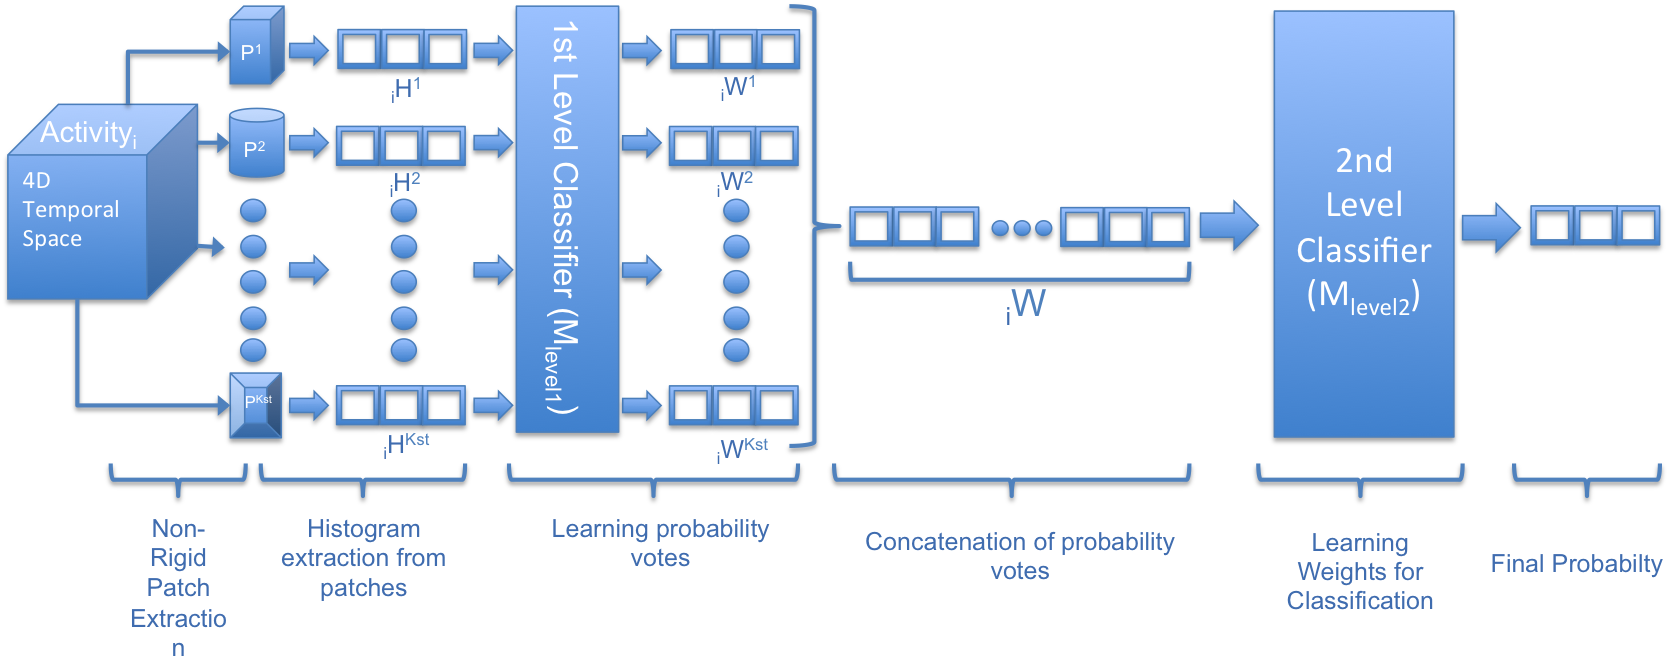
\includegraphics[scale=0.29]{Figures/oneModelApproach3}
\end{center}
\caption{Illustration of one-model approach to classify a video clip \label{fig:oneModelApproachIllustration}}
\end{figure}


\subsubsection{Multi-Model Approach}
\label{section:MultiModelApproach}
In contrast to the one-model approach, we propose to use multiple classifiers in the first level classification. Each patch $P^{j}$ in the first level classification has its own classifier model, i.e., $\{M_{level1}^{1},\dots,M_{level1}^{K_{st}}\}$. In order to train the first level classifiers, $\{M_{level1}^{1},\dots,M_{level1}^{K_{st}}\}$, the training set is separated into $K_{st}$ for each patch type. Each first level classifier, $M_{level1}^{j}$, is trained with its corresponding patch histograms, i.e., $\{_{1}H^{j},...,_{N_{v}}H^{j}\}$ where $N_{v}$ is number of video clip pairs. Then, we use the same training set to test the models to get probability votes, $\{W^{1},...,W^{K_{st}}\}$ where $W^{j} \in \mathbb{R}^{N_{c}}$ and $N_{c}$ is the number of activity classes. Then, we get concatenated probability vector $W$ for each video clip as described in Section~\ref{section:OneModelApproach} and train the second level classifier. Testing is done as follows: (1) testing set is separated according to patch types, (2) each patch type is tested though the corresponding classifier in the first level to get probability votes, (3) histograms from the first level is concatenated and tested against the second level. An illustration of the multi-model approach is shown in Figure~\ref{fig:multiModelApproachIllustration}.
    
    
\begin{figure}[!htbp]
\begin{center}
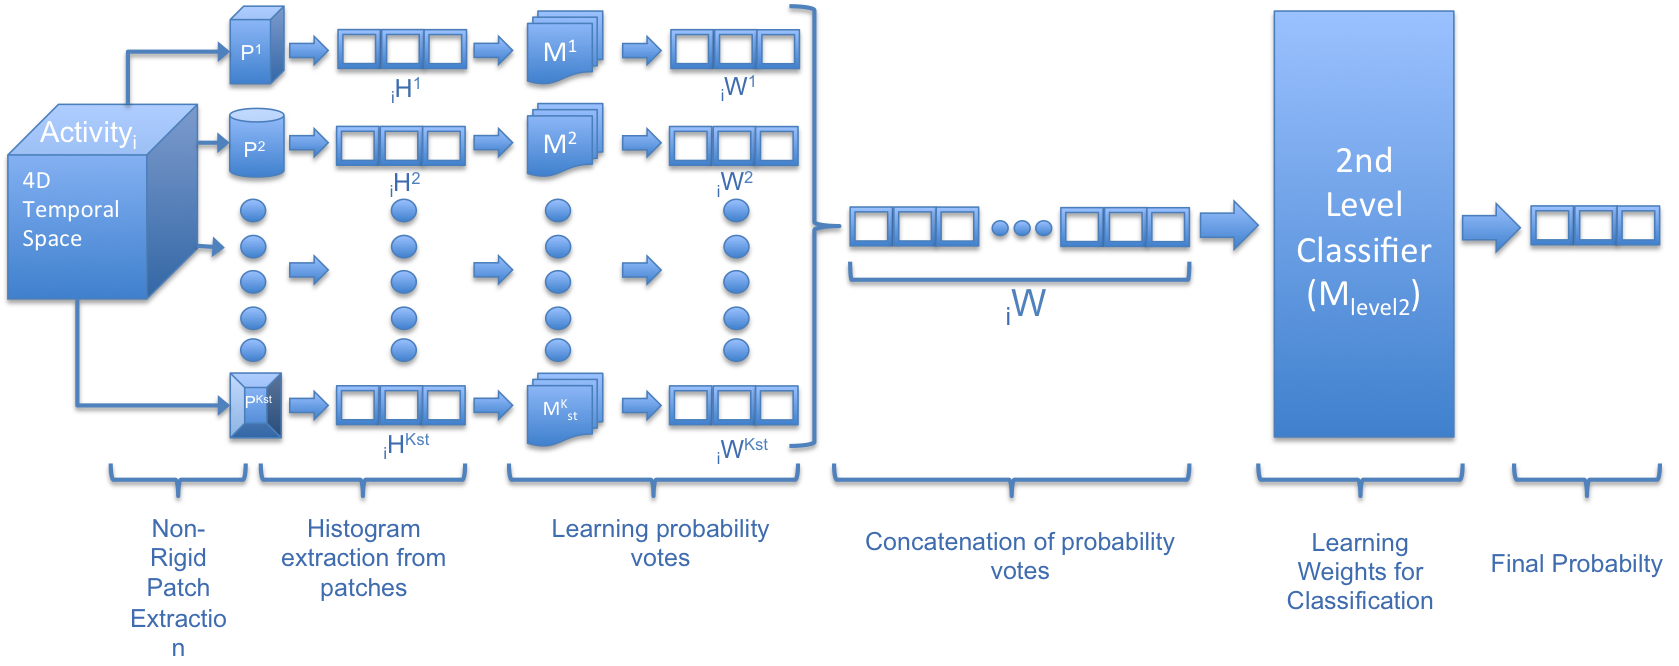
\includegraphics[scale=0.29]{Figures/multiModelApproach3}
\end{center}
\caption{Illustration of multi-model approach to classify a video clip \label{fig:multiModelApproachIllustration}}
\end{figure}
   
%%%%%%%%%%%%%%%%%%%%%%%%%%%%%%%%%%%%%%%%%%%%%%%%%%%%%%%%%%%%%%%%%%%%%%%%%%%%%%%%
\section{EXPERIMENTS}
\label{section:experiments}

% In this chapter, experimental setup and results are described. First, the dataset is explained in detail with quantitative information. Then, feature extraction and encoding parameters and classification setups are shown and explained. Finally, results of evaluation of the proposed voting scheme are presented.

\subsection{Experimental Setup}
\label{section:experimentalSetup}

        In order to evaluate the performance of the proposed voting scheme with data-driven 4D spatio-temporal patches, the dataset collected by \cite{c1} is used. Composed of intensity and depth videos from 2 different views, the dataset has 11 days of recording of the operating room with real surgeries. The dataset is annotated with 15 different general and surgery-specific activities. 
        %The general activities are the common activities taking place in the operating room, e.g., bed entering, moving patient to OR bed, bed leaving, moving patient from OR bed, etc.
        The general activities are the common activities taking place in the OR and
        the surgery-specific activities are picked from vertebroplasty procedures due to its frequency in the dataset. 
%         Vertebroplasty is a surgical procedure to stabilize the spinal fractures in which bone cement is injected through small punctures on the patient's skin to reduce pain. The dataset has 3 vertebroplasty specific activities, i.e., hammering, mixing cement and cement injection. 
        The dataset contains 1734 annotated video clips. Number of instances for each class are shown in Figure~\ref{fig:datasetChart}. Since the dataset is unbalanced as shown in Figure~\ref{fig:datasetChart}, bagging approach is used to balance instances from each class.

\begin{table}[h]
\centering
\begin{tabular}{|c|c|c|}
\hline
{\bf Activity}             & {\bf \#Instance} & {\bf Length (s) (mean $\pm$ std)} \\ \hline
Adjusting C-arm            & 507              & 14.5 $\pm$ 24.3                   \\ \hline
Adjusting OR bed           & 144              & 8.8 $\pm$ 4.9                     \\ \hline
Bed entering               & 59               & 15.8 $\pm$ 7.0                    \\ \hline
Bed leaving                & 61               & 19.9 $\pm$ 9.8                    \\ \hline
Cement injection           & 29               & 374.4 $\pm$ 105.1                 \\ \hline
Cleaning patient’s back    & 245              & 20.0 $\pm$ 10.4                   \\ \hline
Hammering                  & 216              & 15.8 $\pm$ 7.2                    \\ \hline
Monitor adjustment         & 136              & 12.6 $\pm$ 7.7                    \\ \hline
Moving patient from OR bed & 31               & 15.0 $\pm$ 5.1                    \\ \hline
Moving patient to OR bed   & 30               & 20.2 $\pm$ 8.4                    \\ \hline
Putting sterile drapes     & 126              & 10.5 $\pm$ 4.4                    \\ \hline
Removing sterile drapes    & 42               & 17.4 $\pm$ 9.0                    \\ \hline
Mixing cement              & 28               & 75.9 $\pm$ 21.5                   \\ \hline
Opening package            & 51               & 12.7 $\pm$ 5.4                    \\ \hline
Throwing package           & 29               & 10.2 $\pm$ 4.0                    \\ \hline
\end{tabular}
\caption{Dataset Information}
\label{fig:datasetChart}
\end{table}


% \begin{table}[h]
% \centering
% \begin{tabular}{|c|c|}
% \hline
% {\bf Activity}             & {\bf Instance Count} \\ \hline
% Adjusting C-arm            & 507                  \\ \hline
% Adjusting OR bed           & 144                  \\ \hline
% Bed entering               & 59                   \\ \hline
% Bed leaving                & 61                   \\ \hline
% Cement injection           & 29                   \\ \hline
% Cleaning patient’s back    & 245                  \\ \hline
% Hammering                  & 216                  \\ \hline
% Monitor adjustment         & 136                  \\ \hline
% Moving patient from OR bed & 31                   \\ \hline
% Moving patient to OR bed   & 30                   \\ \hline
% Putting sterile drapes     & 126                  \\ \hline
% Removing sterile drapes    & 42                   \\ \hline
% Mixing cement              & 28                   \\ \hline
% Opening package            & 51                   \\ \hline
% Throwing package           & 245                  \\ \hline
% \end{tabular}
% \caption{Dataset Information}
% \label{fig:datasetChart}
% \end{table}
% \begin{center}
% \begin{figure}
% \begin{tikzpicture}[scale=0.4]
% \begin{axis}[
%     xbar,
%     bar width=\baselineskip,
%     xmin=0.0,
%     width=12cm,
%     height=14cm,
%     ytick={1,2,3,4,5,6,7,8,9,10,11,12,13,14,15},
%     yticklabels={{Throwing package},{Opening package},{Mixing cement},{Removing sterile drapes},{Putting sterile drapes},{Moving patient to OR bed},{Moving patient from OR bed},{Monitor adjustment},{Hammering},{Cleaning patient’s back},{Cement injection},{Bed leaving},{Bed entering},{Adjusting OR bed},{Adjusting C-arm}},
%     enlarge y limits=0.1,
%     xlabel={Instance Counts for each Class},
%     ytick=data,
%     nodes near coords,
%     nodes near coords align=left,
%     every node near coord/.style={color=white}
% ]
% \addplot [draw=black, fill=cyan!40!black] coordinates {
%     (245, 1)
%     (51, 2)
%     (28, 3)
%     (42, 4)
%     (126, 5)
%     (30, 6)
%     (31, 7)
%     (136, 8)
%     (216, 9)
%     (245, 10)
%     (29, 11)
%     (61, 12)
%     (59, 13)
%     (144, 14)
%     (507, 15)
% };
% \end{axis}
% \end{tikzpicture}
% \caption{Dataset Information}
% \label{fig:datasetChart}
% \end{figure}
% \end{center}

    	\subsubsection{Visual feature extraction and encoding}
        \label{section:VisualFeatureExtractionAndEncoding}
        In interest point detection, we detect 1000 STIPs from intensity and 1000 DSTIPs from depth data from each video clip. Then, we extract 480-dimensional HOF from intensity and 4005-dimensional DCSF from depth data around each interest point. We use Principal Component Analysis (PCA) to reduce dimensions of HOF and DSCF to 250 and 800 respectively for visual dictionary construction. All these parameters have proven to produce good results in \cite{c1}. 
%         In \cite{twinanda2015data}, performance comparison of size of visual dictionaries are studied and it is shown that visual dictionary size 1500 has the highest accuracy and increasing the number of words in dictionary size has not much improve the performance. 
        Then second dictionary, spatio-temporal dictionary, is built to divide 4D spatio-temporal space into non-rigid cells with 24 patches for intensity and depth data. When we use combination of intensity and depth data, the number of 4D patches becomes 48 (24 from both intensity and depth).

        
        \subsubsection{Classification Setup}
        \label{section:ClassificationStrategy}
        In this work, we use SVM and RF classifiers. In the experiments, two-level classification strategy is used and explained in detail in Section~\ref{section:ActionClassification}. K-Fold cross validation is used to evaluate performance of the classifiers by dividing dataset into 10 folds.
        %We also use two different approaches: one-model and multi-model. In one-model approach, a single classifier model is trained on each level. In contrast, in the multi-model approach, multiple classifier models are trained on the first level. For intensity and depth data, 24 classifier models are trained. However, for the combination, 48 classifier models are trained. These numbers are used to match the number of 4D patches.
        
        
        \subsubsection{SVM Setup}
        \label{section:SVMSetup}
         SVM models in the experiments are trained using VLFeat toolbox \cite{c28}. SVM is used with non-linear kernels, i.e., Chi-square $ \left(\mathcal{X}\right)^{2} $ and histogram intersection kernels. %Since there is 15 different classes for classification, one-against-all SVM is used to handle multi-class problem. K-Fold cross validation is used to evaluate performance by dividing the dataset into 10 folds.
        
        \subsubsection{Random Forest Setup}
        \label{section:RandomForestSetup}
        %RF models in the experiments are trained using our own implementation of RF. RFs depend on many parameters, e.g., number of trees, maximum depth of the trees, minimum information gain and minimum number of samples in each tree node as stopping criteria to stop building a tree. 
        RFs are trained with 100 trees, with maximum depth 15. The minimum information gain in the node is set to 0.001 to avoid trees with low information gain. One of the effective parameter in tree building is the minimum number of samples reach to each node before stopping. We use 32 samples as minimum number of samples in node as stopping criteria. Each tree in the RF have seen 80\% of the training data as randomly for bagging across trees. 
        %Finally K-Fold cross validation is used to evaluate the performance by dividing the dataset into 10 folds.


\subsection{Experimental Results}
\label{section:experimentalResults}

% In this section, we report results from the voting scheme as well as the comparison with non-voting scheme. We also compare the one-model and multi-model approaches using the proposed two-level classification strategy with the voting scheme, and their results compared on intensity, depth and the combination of the intensity and depth.

%     In this section, we conduct experiments to verify and evaluate our proposed voting scheme strategy on the aforementioned dataset \cite{twinanda2015data} and report the results by comparing to non-voting approach \cite{twinanda2015data}. We use intensity, depth and their combination individually for evaluation using two different classifiers, i.e., non-linear SVM and Random Forest. In the experiments we use two different evaluation methods that changes classification strategy: one-model and multi-model strategies that their setup is described in Section~\ref{ClassificationStrategy}. We share results from the one model and multi model under Section~\ref{section:OneModel} and Section~\ref{section:MultiModel} respectively.
    
\subsubsection{One-Model Approach}
\label{section:OneModelExperiments}
%Single SVM and RF models are trained in each level with all patches from each activity. 
In Table~\ref{table:oneModelResults}, results for one-model approach is presented with intensity, depth and combination of the data with both of the classifiers. It is shown that non-linear SVM performs slightly better than the RF. It is also shown that combination of the intensity and depth data has more discriminating power than using only intensity or depth. The combination of the depth and intensity profits the complementary information that intensity and depth carries. Because some activities are well classified in intensity due to illumination and intensity changes, e.g., cement injection, however some actions showed better performance in depth due to high variance in depth, e.g., Adjusting C-Arm. The combination of the intensity and depth data gets the highest accuracy with 83.1\% accuracy using SVM and the confusion matrix is shown in Table~\ref{fig:combinationOneModelConfusionMatrix}.


\begin{table}[h]
\centering
\begin{tabular}{|c|c|c|}
\hline
                     & \textbf{SVM}     & \textbf{RF} \\ \hline
\textbf{Intensity}   & \textbf{74.45\%} & 70.06\%     \\ \hline
\textbf{Depth}       & \textbf{72.72\%} & 67.87\%     \\ \hline
\textbf{Combination} & \textbf{83.1\%}  & 79.18\%     \\ \hline
\end{tabular}
\caption{Classification results using one-model approach}
\label{table:oneModelResults}
\end{table}

% \begin{figure}[H]
% \begin{center}
% 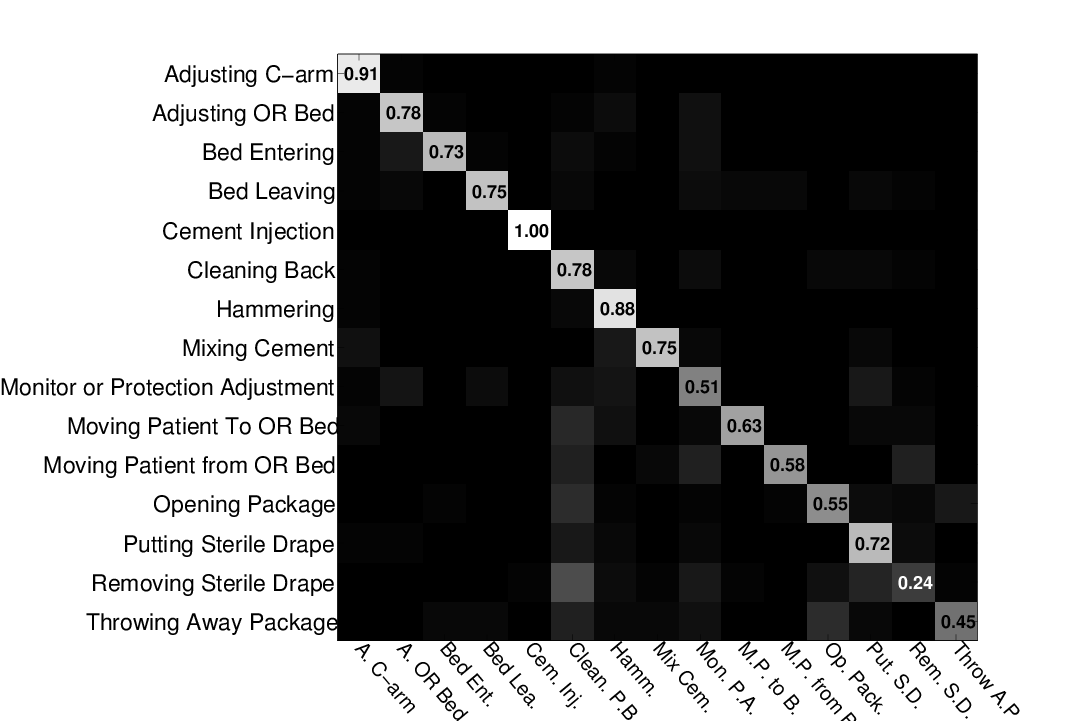
\includegraphics[scale=0.1]{Figures/intensity-onemodel}
% \end{center}
% \caption{Confusion matrix of one-model approach using intensity features \label{fig:intensityOneModelConfusionMatrix}}
% \end{figure}
        
% \begin{figure}[H]
% \begin{center}
% 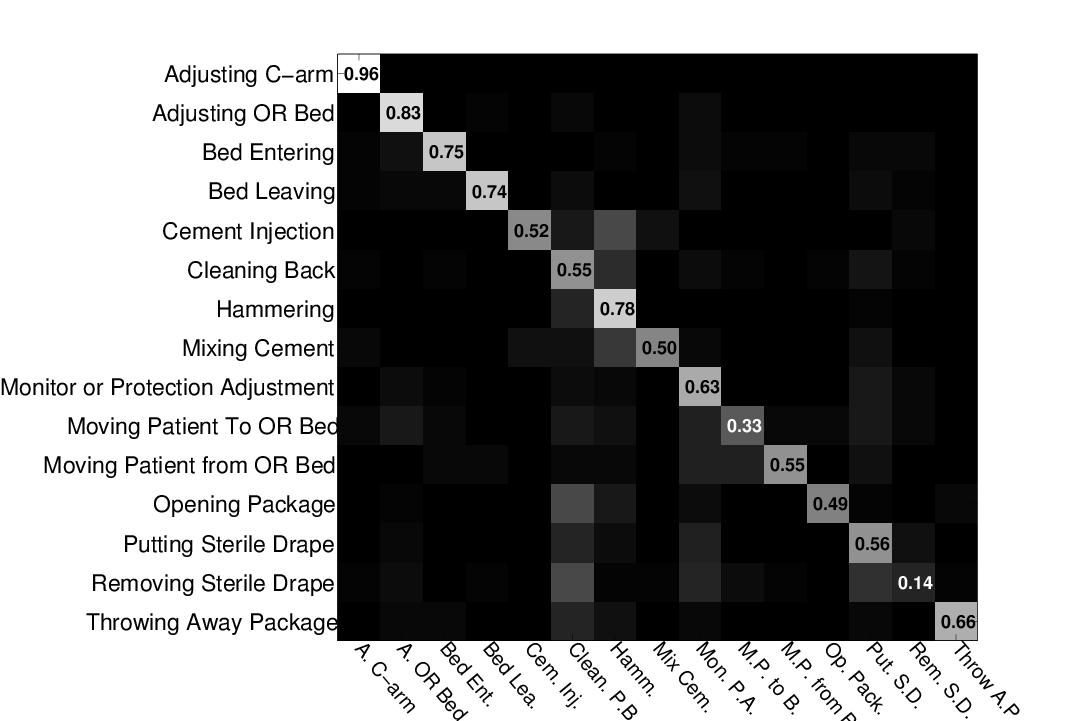
\includegraphics[scale=0.1]{Figures/depth-onemodel}
% \end{center}
% \caption{Confusion matrix of one-model approach using depth features \label{fig:depthOneModelConfusionMatrix}}
% \end{figure}

\begin{figure}[H]%[!htbp]%[here][H]
\begin{center}
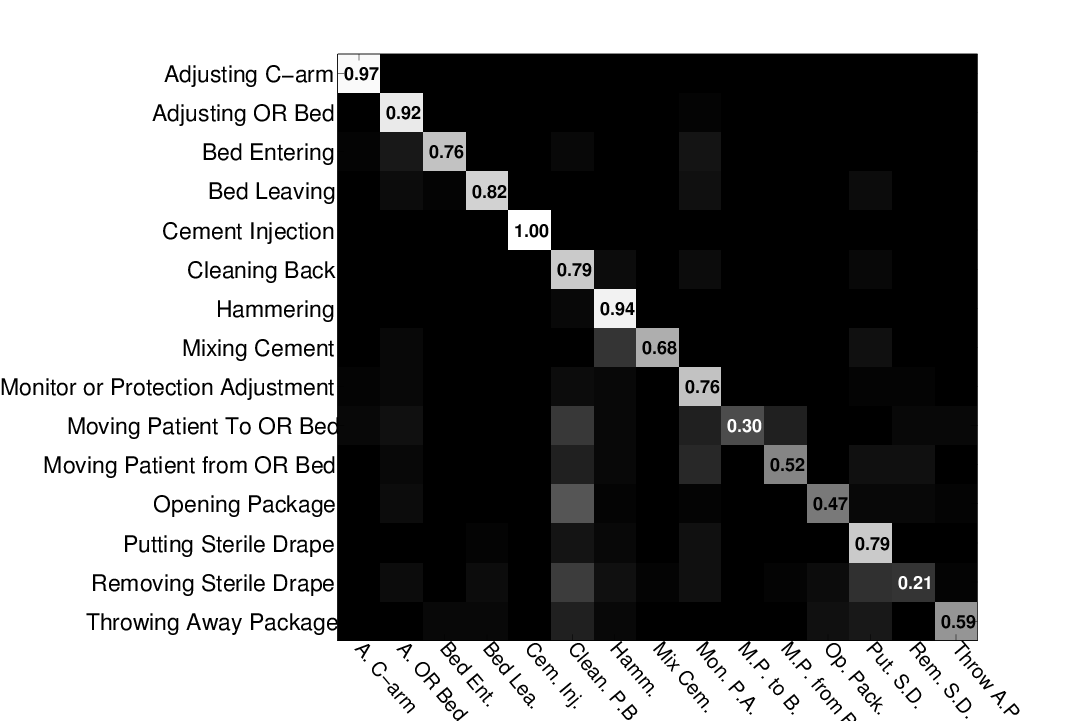
\includegraphics[scale=0.20]{Figures/combination-onemodel}
\end{center}
\caption{Confusion matrix of one-model approach using combination of features
\label{fig:combinationOneModelConfusionMatrix}}
\end{figure}

\subsubsection{Multi-Model}
\label{section:MultiModelExperiments}
In the multi-model approach , we learn multiple models in the first level for each patch type $P^{j}$. In contrast, the one-model approach trained a single model for the first level using all the patches from all the video clips.
Hence, one-model approach profits from seeing more training data whereas in the multi-model approach, the first level classifiers sees less training data. In other words, multi-model has slight disadvantage over one-model approach due to training the each patch model. Thus, results presented in Table~\ref{table:multiModelResults} have slightly lower accuracy than one-model results in Table~\ref{table:oneModelResults}. On the other hand, the combination of intensity and depth is still performing better than using only intensity or depth. We achieved 81.71\% accuracy with combination of the data with the SVM classifier. The detailed results are presented with confusion matrix in \ref{fig:combinationMultiModelConfusionMatrix}.
            
\begin{table}[H]
\centering
\begin{tabular}{|c|c|c|}
\hline
                     & \textbf{SVM}     & \textbf{RF} \\ \hline
\textbf{Intensity}   & \textbf{77.28\%} & 69.20\%     \\ \hline
\textbf{Depth}       & \textbf{71.91\%} & 64.45\%     \\ \hline
\textbf{Combination} & \textbf{81.71\%} & 75.54\%     \\ \hline
\end{tabular}
\caption{Classification results using multi-model approach}
\label{table:multiModelResults}
\end{table}

% \begin{figure}[H]
% \begin{center}
% 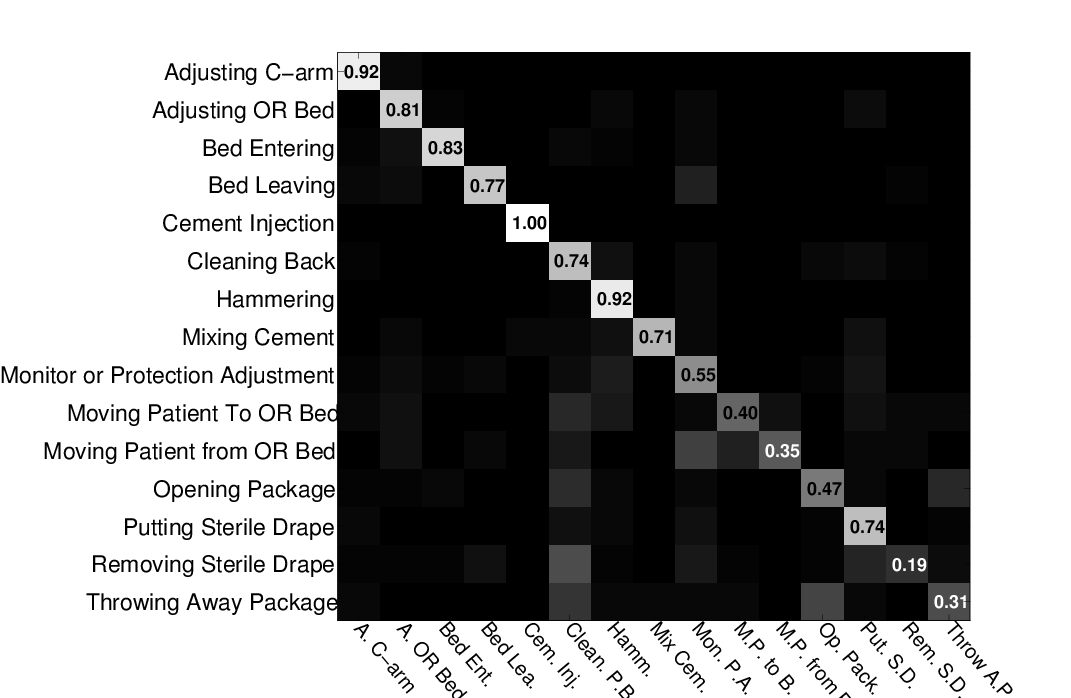
\includegraphics[scale=0.1]{Figures/intensity-multimodel}
% \end{center}
% \caption{Confusion matrix of multi-model approach using intensity features 
% \label{fig:intensityMultiModelConfusionMatrix}}
% \end{figure}
        
% \begin{figure}[H]
% \begin{center}
% 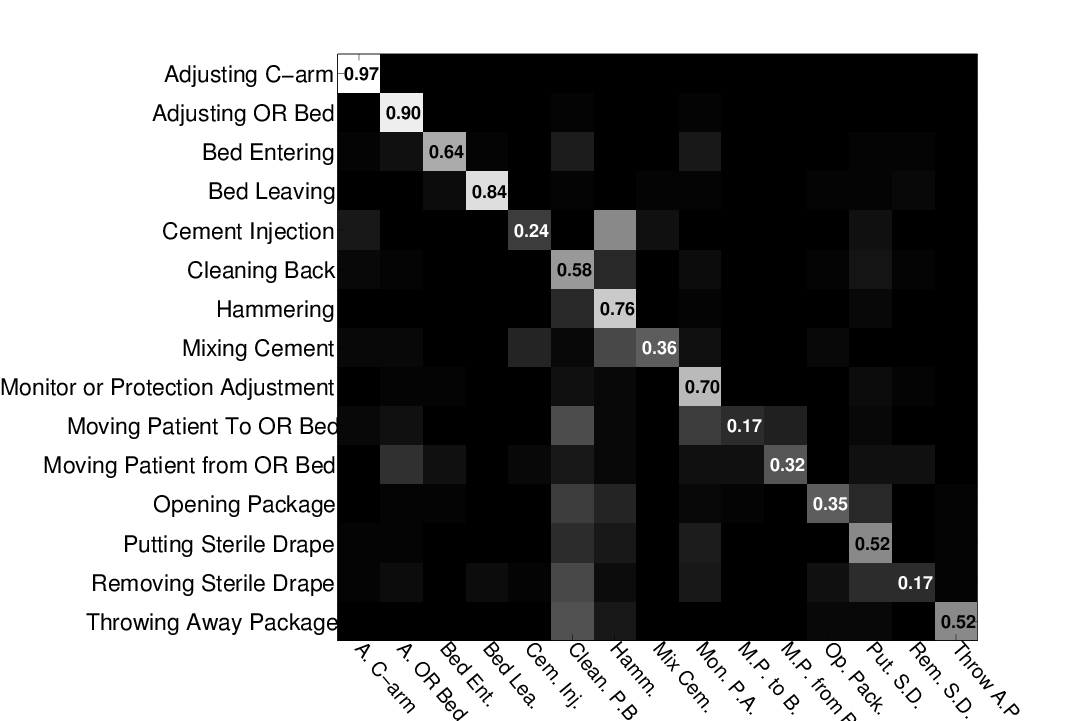
\includegraphics[scale=0.1]{Figures/depth-multimodel}
% \end{center}
% \caption{Confusion matrix of multi-model approach using depth features  
% \label{fig:depthMultiModelConfusionMatrix}}
% \end{figure}

\begin{figure}[H]%[!htbp]%[here][H]
\begin{center}
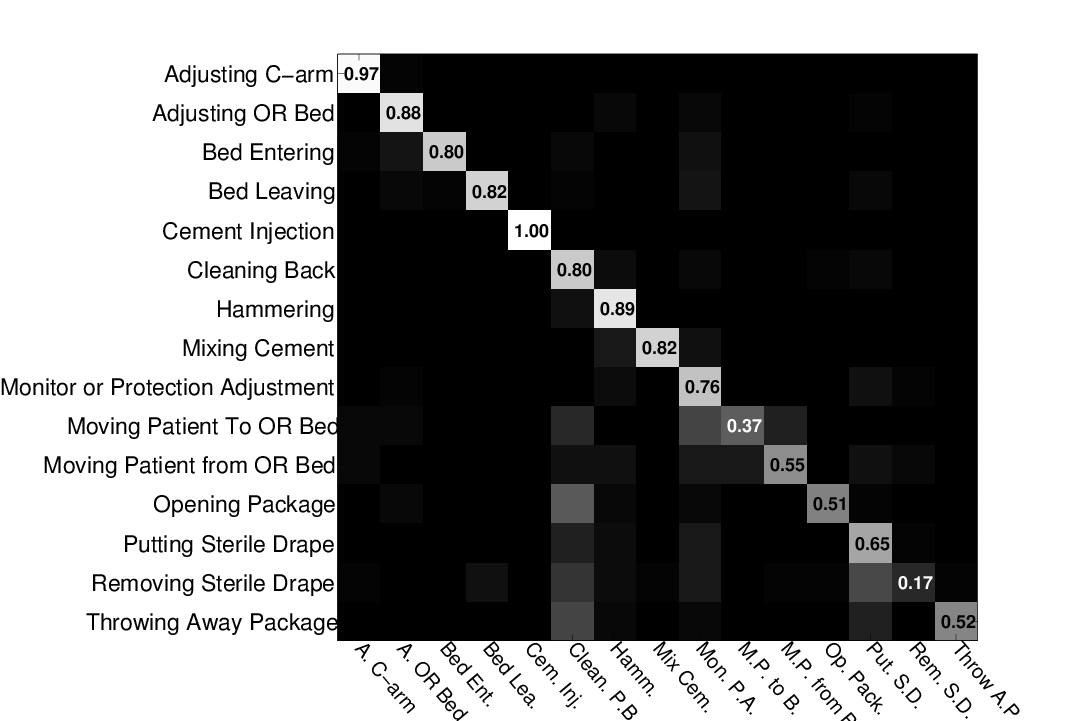
\includegraphics[scale=0.20]{Figures/comb-multimodel}
\end{center}
\caption{Confusion matrix of multi-model approach using combination of features  
\label{fig:combinationMultiModelConfusionMatrix}}
\end{figure}
            
            
            
\subsubsection{Non-Voting Approach}
\label{section:NonVotingAproachExperiments}
	%The proposed voting scheme approach also compared to non-voting scheme approach in \cite{c1}. 
    In \cite{c1}, a data-driven non-rigid layout is used by concatenating the histogram vectors from patches to construct single histogram vector to represent video clip. The histogram vector also concatenated with a histogram vector extracted from video clip without using any layout. Hence, the final concatenated histogram carries more information than using histograms from each patch separately as in Section~\ref{section:OneModelExperiments} and Section~\ref{section:MultiModelExperiments}. Using the patch histograms separately for training and collecting votes increased the sparsity problem in classification in the first level. The non-voting method reached 85.53\% accuracy compared to our maximum accuracy 83.1\%. The detailed comparison with intensity, depth data and their combination is shown in Table~\ref{table:comparisonResults}.
    
    
\begin{table}[H]
\centering
\begin{tabular}{|c|c|c|}
\hline
                  & {\bf Non-Voting \cite{c1}}   & {\bf Voting} \\ \hline
{\bf Intensity}   & {\bf 80.40\%} & 74.45\%    \\ \hline
{\bf Depth}       & {\bf 78.37\%} & 72.72\%    \\ \hline
{\bf Combination} & {\bf 85.53\%} & 83.1\%     \\ \hline
\end{tabular}
\caption{Classification accuracy comparison of non-voting \cite{c1} and voting scheme}
\label{table:comparisonResults}
\end{table}
           

% \begin{figure}[H]%[!htbp]%[here][H]
% \begin{center}
% 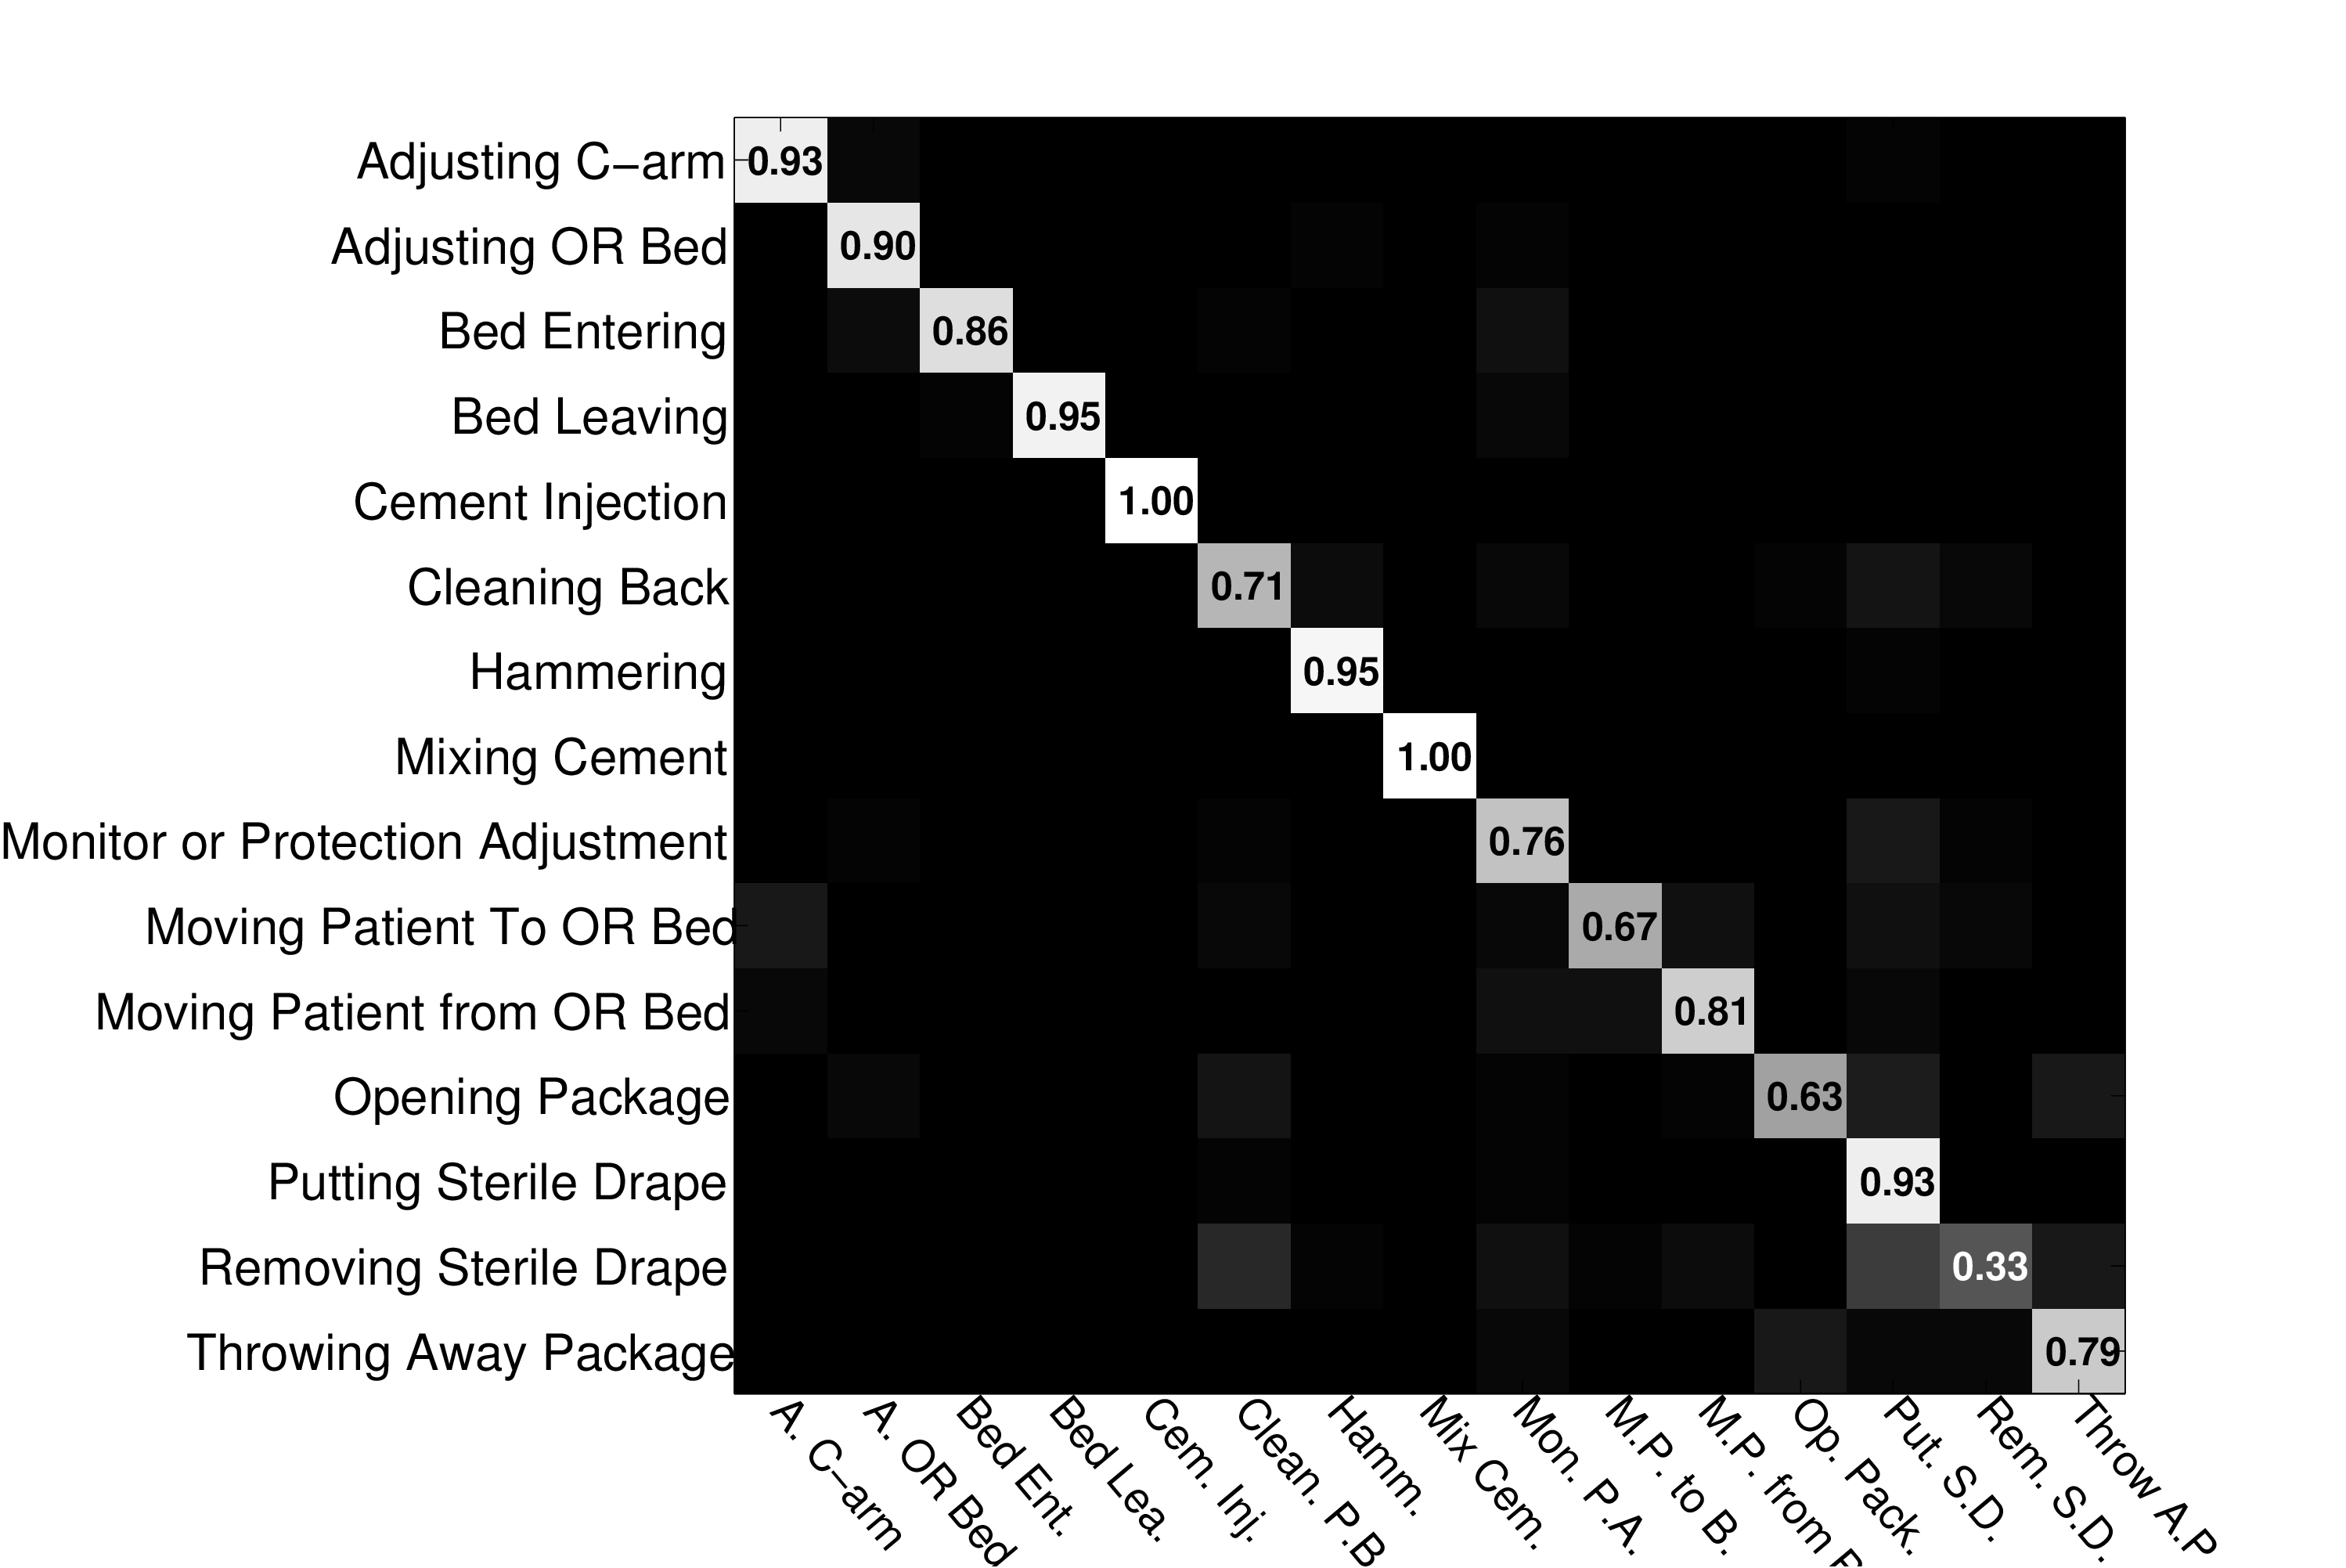
\includegraphics[scale=0.06]{Figures/confusionAndruPaper1}
% \end{center}
% \caption{Confusion matrix of non-voting scheme using combination of features\cite{c1} 
% \label{fig:combinationNonVotingConfusionMatrix}}
% \end{figure}

The voting scheme has better detection on activities, i.e., Adjusting C-Arm, Adjusting OR Bed and Cleaning Back, where in these activities, detected interest points are more separable and informative than other activities. For example, in  Mixing Cement activity, 32\% accuracy decreased in voting scheme approach. In this activity, interest points are detected in very narrow space, and they detected as cluster around the activity. Thus, detected interest points are not uniform in 4D space but distributed around one point. The decrease in the accuracy can be explained as the detected interest points in 4D space is not separated informatively with non-rigid layout for the Mixing Cement activity.

% In comparison of confusion matrices with voting and non-voting scheme from  Figure~\ref{fig:combinationOneModelConfusionMatrix} and Figure~\ref{fig:combinationNonVotingConfusionMatrix}, it is shown that the voting scheme has better detection on activities, i.e., Adjusting C-Arm, Adjusting OR Bed and Cleaning Back, where in these activities, detected interest points are more separable and informative than other activities. For example, in  Mixing Cement activity, 32\% accuracy decreased in voting scheme approach. In this activity, interest points are detected in very narrow space, and they detected as cluster around the activity. Thus, detected interest points are not uniform in 4D space but distributed around one point. The decrease in the accuracy can be explained as the detected interest points in 4D space is not separated informatively with non-rigid layout for the Mixing Cement activity.

%%%%%%%%%%%%%%%%%%%%%%%%%%%%%%%%%%%%%%%%%%%%%%%%%%%%%%%%%%%%%%%%%%%%%%%%%%%%%%%%
\section{CONCLUSIONS}
\label{section:conclusionsAndFutureWorks}

% \subsection{Conclusions}
% \label{section:conclusions}

	In this paper, a voting scheme approach is proposed to address the problem of activity recognition in an operating room using a multi-view RGBD camera system. The 4D spatio-temporal space is divided into smaller local patches using a data-driven non-rigid layout by \cite{c1} which also helps with sparse interest points. A two-level classification strategy is introduced, i.e., learning the probability votes and learning the weights. Furthermore, two different classification approaches are compared using two-level classification: one-model and multi-model. The one-model approach performed better than the multi-model. Voting scheme showed promising results with 83.1\% accuracy.
    
    %The one-model approach trained a single classifier model with all patches from the all video clips in each level, however, the multi-model approach trained separate classifier models for  each patch type in a video clip in the fist level. Finally, the proposed voting strategy collects votes from the each local patch from a video clip and the weights are used to recognize the activity. The voting scheme is evaluated on a new dataset from \cite{c1} which consists of annotated 1734 real surgical video clips with 15 different surgical activity types. In order to make comprehensive comparison, we compared the proposed voting scheme with non-voting scheme approach from \cite{c1}. We have shown that the proposed voting scheme gives promising results. 


% \subsection{Future Works}
% \label{section:futureWorks}

    The current STIP detection is based on movements occur in the video clips where the detection is in the borders of the action. Hence, the detected interest points are sparse and ignore the information from stationary parts of the videos. Additionally, the BoW approach is another limit which encodes the features into sparse representation. It would be interesting to incorporate extraction of dense features and different feature encoding approaches. Since the voting scheme uses local parts of 4D spatio-temporal space, it would be interesting to use the voting scheme to recognize concurrent activities.

%%%%%%%%%%%%%%%%%%%%%%%%%%%%%%%%%%%%%%%%%%%%%%%%%%%%%%%%%%%%%%%%%%%%%%%%%%%%%%%%
% \section{ACKNOWLEDGMENTS}
% \label{section:acknowledgments}

% The authors gratefully acknowledge the contribution of National Research Organization and reviewers' comments.


%%%%%%%%%%%%%%%%%%%%%%%%%%%%%%%%%%%%%%%%%%%%%%%%%%%%%%%%%%%%%%%%%%%%%%%%%%%%%%%%

% References are important to the reader; therefore, each citation must be complete and correct. If at all possible, references should be commonly available publications.

% \label{Bibliography}

% \section*{REFERENCES}
% %\lhead{\emph{REFERENCES}} % Change the page header to say "Bibliography"

% \bibliographystyle{unsrtnat} % Use the "unsrtnat" BibTeX style for formatting the Bibliography

% \bibliography{Bibliography} % The references (bibliography) information are stored in the file named "Bibliography.bib"

\begin{thebibliography}{99}


\bibitem{c1}
A. P. Twinanda, E. O. Alkan, A. Gangi, M. de Mathelin, and N.
Padoy. Data-driven spatio-temporal rgbd feature encoding for action recognition in operating rooms. International journal of computer assisted radiology and surgery, pages 1–11, 2015.
%---------------------------%
\bibitem{c2}
B. Bhatia, T. Oates, Y. Xiao, and P. Hu. Real-time identification of operating room state from video. In Proceedings of the 19th National Conference
on Innovative Applications of Artificial Intelligence - Volume 2, IAAI’07, pages 1761–1766. AAAI Press, 2007. 
%ISBN 978-1-57735-323-2. URL http://dl.acm.org/citation.cfm?id=1620113.1620126.
%---------------------------%
% \bibitem{c3}
% F. Lalys, L. Riffaud, D. Bouget, and P. Jannin. A framework for
% the recognition of high-level surgical tasks from video images for cataract surgeries. IEEE Trans. Biomed. Engineering, 59(4):966–976, 2012. 
%doi: 10.1109/TBME.2011.2181168. URL http://dx.doi.org/10.1109/TBME.2011.2181168.
%---------------------------%
\bibitem{c4}
N. Padoy, T. Blum, S. Ahmadi, H. Feussner, M. Berger, and N. Navab. Statistical modeling and recognition of surgical workflow. Medical Image Analysis, 16(3):632 – 641, 2012.
%ISSN 1361-8415. doi: http://dx.doi.org/10.1016/j.media.2010.10.001. URL http://www.sciencedirect.com/science/article/pii/S1361841510001131. Computer As-sisted Interventions.
%---------------------------%
\bibitem{c5}
L. Zappella, B. Bejar, G. Hager, and R. Vidal. Surgical gesture classification from video and kinematic data. Medical Image Analysis, 17(7):732 – 745, 2013.

 %ISSN 1361-8415. doi: http://dx.doi.org/10.1016/j.media.2013.04.007. URL http://www.sciencedirect.com/science/article/pii/S1361841513000522. Special Issue on the 2012 Conference on Medical Image
%Computing and Computer Assisted Intervention.
%---------------------------%
\bibitem{c6}
I. Chakraborty, A. Elgammal, and R.S. Burd. Video based activity recognition
in trauma resuscitation. In Automatic Face and Gesture Recognition (FG), 2013
10th IEEE International Conference and Workshops on, pages 1–8, April 2013.
%doi: 10.1109/FG.2013.6553758.
%---------------------------%
\bibitem{c7}
N. Loy Rodas and N. Padoy. Seeing is believing: increasing intraoperative awareness to scattered radiation in interventional procedures by combining augmented reality, monte carlo simulations and wireless dosimeters. International Journal of Computer Assisted Radiology and Surgery, pages 1–11, 2015. %ISSN 1861-6410. doi: 10.1007/s11548-015-1161-x. URL http://dx.doi.org/10.1007/s11548-015-1161-x.
%---------------------------%
\bibitem{c8}
S. Lazebnik, C. Schmid, and J. Ponce. Beyond bags of features: Spatial pyramid
matching for recognizing natural scene categories. In Computer Vision and Pattern Recognition, 2006 IEEE Computer Society Conference on, volume 2, pages 2169–2178, 2006. %doi: 10.1109/CVPR.2006.68.
%---------------------------%
\bibitem{c9}
L. Xia and J.K. Aggarwal. Spatio-temporal depth cuboid similarity feature for
activity recognition using depth camera. In Computer Vision and Pattern Recog-
nition (CVPR), 2013 IEEE Conference on, pages 2834–2841, June 2013. 
%doi:10.1109/CVPR.2013.365.
%---------------------------%
\bibitem{c10}
H. Wang, A. Klaser, C. Schmid, and C. Liu. Action recognition by dense
trajectories. In Computer Vision and Pattern Recognition (CVPR), 2011 IEEE
Conference on, pages 3169–3176, June 2011. %doi: 10.1109/CVPR.2011.5995407.
%---------------------------%
\bibitem{c11}
X. Yang and Y. Tian. Super normal vector for activity recognition
using depth sequences. In Computer Vision and Pattern Recognition (CVPR),
2014 IEEE Conference on, pages 804–811, June 2014. %doi: 10.1109/CVPR.2014.108.
%---------------------------%
\bibitem{c12}
A. Klaser, M. Marszalek, C. Schmid, and A. Zisserman.
Human focused action localization in video. In Proceedings of the 11th Euro-
pean Conference on Trends and Topics in Computer Vision - Volume Part I, ECCV’10, pages 219–233, Berlin, Heidelberg, 2012. Springer-Verlag. 
%ISBN 978-3-642-35748-0. doi: 10.1007/978-3-642-35749-7 17. URL http://dx.doi.org/10.1007/978-3-642-35749-7_17.
%---------------------------%
\bibitem{c13}
Y. Lin, J. Hua, N.C. Tang, M. Chen, and H.-Y.M. Liao. Depth
and skeleton associated action recognition without online accessible rgb-d cameras. In Computer Vision and Pattern Recognition (CVPR), 2014 IEEE Conference on, pages 2617–2624, June 2014. %doi: 10.1109/CVPR.2014.335.
%---------------------------%
% \bibitem{c14}
% R. Vemulapalli, F. Arrate, and R. Chellappa. Human action recognition by rep-
% resenting 3d skeletons as points in a lie group. In Computer Vision and Pattern Recognition (CVPR), 2014 IEEE Conference on, pages 588–595, June 2014. 
% %doi:10.1109/CVPR.2014.82.
%---------------------------%
% \bibitem{c15}
% D. Wu and L. Shao. Leveraging hierarchical parametric networks for skeletal
% joints based action segmentation and recognition. In Computer Vision and Pattern Recognition (CVPR), 2014 IEEE Conference on, pages 724–731, June 2014. 
% %doi:10.1109/CVPR.2014.98.
%---------------------------%
% \bibitem{c16}
% W. Li, Z. Zhang, and Z. Liu. Action recognition based on a bag
% of 3d points. In Computer Vision and Pattern Recognition Workshops (CVPRW),
% 2010 IEEE Computer Society Conference on, pages 9–14, June 2010. 
% %doi: 10.1109/CVPRW.2010.5543273.
%---------------------------%
\bibitem{c17}
O. Oreifej and Z. Liu. Hon4d: Histogram of oriented 4d normals for activity
recognition from depth sequences. In Computer Vision and Pattern Recognition
(CVPR), 2013 IEEE Conference on, pages 716–723, June 2013. 
%doi: 10.1109/CVPR.2013.98.
%---------------------------%
% \bibitem{c18}
% J. Wang, Z. Liu, J. Chorowski, Z. Chen, and Y. Wu. Robust 3d action recognition with random occupancy patterns. In Proceedings of the 12th European Conference on Computer Vision - Volume Part II, ECCV’12,
% pages 872–885, Berlin, Heidelberg, 2012. Springer-Verlag. 
% %ISBN 978-3-642-33708-6. doi: 10.1007/978-3-642-33709-3 62.
% %URL http://dx.doi.org/10.1007/978-3-642-33709-3_62.
%---------------------------%
% \bibitem{c19}
% J. Wang, Z. Liu, Y. Wu, and J. Yuan. Mining actionlet ensemble for action recognition with depth cameras. In Computer Vision and Pattern Recognition (CVPR), 2012 IEEE Conference on, pages 1290–1297, June 2012. 
% %doi:10.1109/CVPR.2012.6247813.
%---------------------------%
\bibitem{c20}
J. Wang, X. Nie, Y. Xia, Y. Wu, and S. Zhu. Cross-view action modeling, learning, and recognition. In Computer Vision and Pattern Recognition (CVPR), 2014 IEEE Conference on, pages 2649–2656, June 2014. 
%doi:10.1109/CVPR.2014.339.
%---------------------------%
% \bibitem{c21}
% A. Kadkhodamohammadi, A. Gangi, M. de Mathelin, and N. Padoy. Temporally consistent 3d pose estimation in the interventional room using discrete mrf optimization over rgbd sequences. Information Processing in Computer-Assisted Interventions, volume 8498 of Lecture Notes in Computer Science, pages 168–177. Springer International Publishing, 2014. 
% %ISBN 978-3-319-07520-4. doi: 10.1007/978-3-319-07521-1 18. 
% %URL http://dx.doi.org/10.1007/978-3-319-07521-1_18.
%---------------------------%
\bibitem{c22}
F. Zhu, L. Shao, and M. Lin. Multi-view action recognition using local similarity random forests and sensor fusion. Pattern Recognition Leters, 34(1):20 – 24, 2013.

%---------------------------%
% \bibitem{c23}
% D. Weinland, R. Ronfard, and E. Boyer. Free viewpoint action recognition using motion history volumes. Computer Vision and Image Understanding, 104(2-3):249–257, 2006.
%---------------------------%
\bibitem{c24}
D. Weinland, M. Ozuysal, and P. Fua. Making action recognition robust to occlusions and viewpoint changes. In European Conference on Computer
Vision, 2010.
%---------------------------%
% \bibitem{c25}
% I. Laptev. On space-time interest points. International Journal of Computer
% Vision, 64(2-3):107–123, 2005.
%---------------------------%
\bibitem{c26}
P. Dollar, V. Rabaud, G. Cottrell, and S. Belongie. Behavior recognition via
sparse spatio-temporal features. In Visual Surveillance and Performance Evaluation of Tracking and Surveillance, 2005. 2nd Joint IEEE International Workshop on, pages 65–72, Oct 2005. %doi: 10.1109/VSPETS.2005.1570899.
%---------------------------%
\bibitem{c27}
F. Barrera and N. Padoy. Piecewise planar decomposition of 3d point clouds
obtained from multiple static rgb-d cameras. In 3D Vision (3DV), 2014 2nd International Conference on, volume 1, pages 194–201, Dec 2014. 
%doi: 10.1109/3DV.2014.57.
%---------------------------%
\bibitem{c28}
A. Vedaldi and B. Fulkerson. Vlfeat: An open and portable library of
computer vision algorithms. In Proceedings of the International Conference on
Multimedia, MM ’10, pages 1469–1472, New York, NY, USA, 2010. ACM. 
%ISBN 978-1-60558-933-6. %doi: 10.1145/1873951.1874249. 
%URL http://doi.acm.org/10.1145/1873951.1874249.
%---------------------------%


\end{thebibliography}

\end{document}